\documentclass[11pt]{article}

% ArXiv-compatible packages (same preamble as the MicroSims paper)
\usepackage[utf8]{inputenc}
\usepackage[T1]{fontenc}
\usepackage{lmodern}
\usepackage{textcomp}
\usepackage{amsmath,amssymb,amsfonts}
\usepackage{graphicx}
\usepackage[hidelinks]{hyperref}
\usepackage{url}
\usepackage{booktabs}
\usepackage{array}
\usepackage{tabularx}
\usepackage{listings}
\usepackage{xcolor}
\usepackage{algorithm}
\usepackage{algpseudocode}
\usepackage{caption}
\usepackage{subcaption}

% Page geometry
\usepackage[margin=1in]{geometry}
\setlength{\emergencystretch}{3em}  % let lines with long model names stretch instead of overflowing

% Code listing settings
\lstset{
    basicstyle=\small\ttfamily,
    commentstyle=\color{green!50!black},
    numbers=none,
    backgroundcolor=\color{gray!5},
    showspaces=false,
    showstringspaces=false,
    frame=single,
    tabsize=2,
    captionpos=b,
    breaklines=true,
    breakatwhitespace=false
}

% Model names: monospaced, and allowed to break after hyphens so that long
% names do not run into the margin.
\newcommand{\mdl}[1]{\texttt{#1}}
\newcommand{\Qeight}{\mdl{qwen3.8:27b}}
\newcommand{\Gthirtyone}{\mdl{gemma4:31b}}
\newcommand{\Muse}{\mdl{muse-\allowbreak glimmer:30b}}
\newcommand{\Qsix}{\mdl{qwen3.6:35b}}
\newcommand{\Gtwentysix}{\mdl{gemma4:26b}}
\newcommand{\Nemo}{\mdl{nemotron-\allowbreak 3.5-\allowbreak lightning:30b}}
\newcommand{\Mistral}{\mdl{mistral-\allowbreak medium-\allowbreak 3.5:128b}}
\newcommand{\Gptoss}{\mdl{gpt-oss:120b}}
\newcommand{\Devstral}{\mdl{devstral-\allowbreak small-2:24b}}
\newcommand{\Granite}{\mdl{granite4.2:30b}}

% Title and author
\title{Small Language Models as Textbook Generators: A Local-Hardware Benchmark on the NVIDIA DGX Spark and the Intelligent Textbook That Teaches It}

\author{
    Dan McCreary \\
    \texttt{https://www.linkedin.com/in/danmccreary/}
}

\date{Version 0.01 \\ \today}

\begin{document}

\maketitle

% Abstract
\begin{abstract}
Intelligent textbooks---interactive books organized around a graph of concept dependencies---are generated today almost entirely by cloud-hosted frontier models driven by agent skills. This paper asks whether open-weight models small enough to run on one 128~GB desktop workstation can do the same work without sending a token to the cloud. We contribute (1)~a reproducible three-stage benchmark (learning graph, chapter structure, chapter text) on a fixed Algebra~I course description, run through the agent harness and skills that produced the published reference book; (2)~a first single-run measurement of ten open-weight models of 24 to 128 billion parameters on a DGX Spark-class machine; (3)~a deterministic, model-free chapter-conformance score that favors consistency over peak quality; (4)~a cost model checked against measured run times; and (5)~a 23-chapter open textbook, with 506 concepts in a dependency graph, that teaches the method, including how to publish results without exposing the machine tested. Six of ten models produced a learning graph and ran all three stages, but only two wrote every chapter they had designed; the model with the cleanest learning graph was the slowest and wrote no chapter. Conformance scores ranged from 39.0 to 64.3 of 100, and the top two books swap places in 39\% of reweighted trials. Three stages took 1.8 to 5.6 machine hours. All results are single runs, no person has yet judged whether the chapters are correct, and no cloud baseline exists, so we report what completes, not what teaches best.
\end{abstract}


% Main content sections
\section{Introduction}
\label{sec:intro}

\subsection{An Empirical Question}

A textbook that carries its own interactive simulations, quizzes, glossary, and a machine-readable map of which concept depends on which is now within reach of a single author working with a generative AI assistant \cite{brusilovsky2022return, mccreary2025microsims}. The assistant is usually a frontier model hosted by a cloud provider. That arrangement is convenient, and it has four costs that a growing number of organizations weigh: the source material and the generated text pass through a third party; the model, its price, and its behavior can change without notice; a long generation job is subject to rate limits however much the customer is willing to pay; and the author's prompts and tooling drift toward one vendor's conventions.

The hardware picture has shifted in parallel. A class of desktop systems built on a single system-on-chip with 128~GB of unified CPU--GPU memory, of which the NVIDIA DGX Spark is the best known \cite{nvidia2025dgxspark}, can hold open-weight models of up to roughly one hundred billion parameters. Position papers argue that small language models (SLMs) are sufficient, better suited, and cheaper for many repetitive agentic tasks \cite{belcak2025slm}. Whether that claim holds for a task as long-horizon and format-sensitive as writing a textbook is an empirical question, and it is the question this paper asks:

\begin{quote}
\textit{Can a single DGX-class workstation, running an open-weight small language model under the same agent harness and skills used for cloud generation, produce an intelligent textbook from a course description without sending a token off the machine?}
\end{quote}

\subsection{Why the Task Is Harder Than It Looks}

Textbook generation is often imagined as a long-form writing problem. In practice, the workload we study is closer to a long-horizon software task. A \textit{skill} is a document of a thousand lines or more that tells an agent what to do, with reference files, templates, and scripts beside it that the agent must find and use at the right step \cite{anthropic2025skills}. A single stage takes tens of tool calls. The output of each stage is the input to the next, and the files passed between stages (CSV, JSON, YAML, Markdown with embedded specifications) must be well formed or the next stage fails. A model that writes good prose but emits a tool call as plain text, loses the thread of a long instruction, or takes ninety minutes per turn will not finish. The benchmark therefore stresses two abilities above all: following a long skill faithfully, and calling tools correctly dozens of times in one session.

\subsection{Approach and Contributions}

We built an evaluation around a published, cloud-generated Algebra~I textbook, restricted to the first three stages of the generation pipeline, and ran it through a local harness on one DGX-class machine. The same effort produced a second artifact: an open, 23-chapter intelligent textbook that teaches how to run such an evaluation. This paper describes both. Its contributions are:

\begin{enumerate}
\item \textbf{A reproducible benchmark definition.} A fixed course description, one fixed prompt per stage, pinned harness and server versions, fresh workspaces, and explicit time limits, so that the model is the only thing that changes (Section~\ref{sec:design}).

\item \textbf{A first measurement of ten open-weight models.} Six produced a learning graph and ran all three stages; two wrote every chapter they designed. We give completion, time, tool-call behavior, and a taxonomy of the failures observed (Section~\ref{sec:results}).

\item \textbf{A deterministic chapter-conformance score.} A 0--100 score computed from counts a program can reproduce, with no model as judge, built to favor consistent quality over peak quality, with its own validation limits stated (Section~\ref{sec:measurement}).

\item \textbf{A cost model checked against measurement.} The model's per-hour cost and its predicted run times are compared with the wall-clock time of the runs (Section~\ref{sec:cost}).

\item \textbf{An open textbook that teaches the method.} 23 chapters, 506 concepts with 824 dependencies, 36 MicroSims, a glossary, quizzes, and annotated references, generated with the same skill chain it evaluates (Section~\ref{sec:book}).

\item \textbf{A publication discipline for private hardware.} A practice for publishing results from a machine that must stay hard to find, reach, and log in to (Section~\ref{sec:publishing}).
\end{enumerate}

\subsection{Scope and Honesty About What Is Known}

This is a first round. Every model ran each stage once. No person has yet judged whether any generated chapter is mathematically correct or pedagogically sound. The cloud baseline has not been run. The conformance score measures adherence to written rules, not truth, and has not been compared with human ratings. We state these limits early because they bound every claim that follows: the paper reports what \textit{completes} and what a program can \textit{count}, not which model teaches best.

\subsection{Paper Organization}

Section~\ref{sec:related} places the work among intelligent-textbook research, SLM and local-inference work, agent harnesses, and language-model evaluation. Section~\ref{sec:book} describes the textbook itself. Section~\ref{sec:design} defines the benchmark, the roles, the hardware, the models, and the controls. Section~\ref{sec:measurement} describes structural checks and the conformance score. Section~\ref{sec:results} reports results. Section~\ref{sec:cost} gives the cost model. Section~\ref{sec:publishing} describes how results were published safely. Section~\ref{sec:discussion} discusses findings, implications, and threats to validity, and Section~\ref{sec:conclusion} concludes.

\section{Background and Related Work}
\label{sec:related}

\subsection{Intelligent Textbooks and Learning Graphs}

Intelligent textbooks have a history reaching back to adaptive hypermedia in the early 1990s. Brusilovsky, Sosnovsky, and Thaker trace several generations, from hand-built domain models to interaction data mining, and note that the line of work never stopped even as attention to it waxed and waned \cite{brusilovsky2022return}. The book evaluated here uses a simple five-level scale: static content, interactive content (hyperlinks, quizzes, simulations, glossary), adaptive content, chatbot integration, and autonomous AI that generates lessons for each reader. The books the benchmark generates are Level~2.

The structural device that makes generation tractable is the \textit{learning graph}: a directed acyclic graph of concepts in which an edge means ``must be understood before.'' The idea sits in a long line of work on prerequisite structure, from knowledge spaces, in which a prerequisite partial order defines the states of knowledge a learner can be in \cite{doignon1999knowledge}, to concept maps, in which concepts joined by labeled links form propositions around a focus question \cite{novak2008concept}. A learning graph also supports a mechanical quality check, since a valid graph has no cycle, and a mechanical ordering, since any topological order is a legal chapter order. Learning outcomes and quiz items are labeled with the revised Bloom taxonomy \cite{anderson2001taxonomy}, and the course description that seeds the pipeline follows backward design: results first, then evidence, then lessons \cite{wiggins2005ubd}.

Interactive elements in the pipeline are MicroSims: small, browser-based simulations, each tied to one concept, embedded by iframe, and specified in a standard layout so that a language model can generate and revise them \cite{mccreary2025microsims}. This paper does not evaluate MicroSim generation; it is the stage the benchmark deliberately leaves out (Section~\ref{sec:design}).

\subsection{Small Language Models and Local Inference}

``Small'' has no fixed meaning. Surveys of small language models typically concern models of 100 million to a few billion parameters \cite{lu2024slm, wang2024slmsurvey}. Belcak et~al.\ instead define an SLM functionally, as a model that can run on a common consumer device with latency low enough to serve one user's agentic requests \cite{belcak2025slm}. We follow the functional reading, as does the book: an SLM is \textit{a model small enough to run on one machine you control}. On the machine tested here, that admits models of 24 to 128 billion total parameters, many of which are sparse mixtures of experts \cite{shazeer2017moe} that activate only 3 to 5 billion parameters per token; \texttt{gpt-oss-120b}, for example, has about 117 billion parameters of which 5.1 billion are active for each token \cite{openai2025gptoss}. This is large by the standard of the surveys and small beside frontier systems, and we use ``SLM'' in this operational sense throughout.

Three technical facts make the 128~GB class workable. Weight quantization shrinks a model to a fraction of its 16-bit size with modest quality loss \cite{dettmers2022llmint8, frantar2022gptq}; every model tested here ran at its publisher's default 4-bit file. Sparse mixtures of experts read only the active experts for each token, which raises decode speed on bandwidth-limited hardware. And unified memory lets weights and conversation context share one pool, so that a long context competes directly with the weights rather than spilling to a separate device memory \cite{nvidia2025dgxspark}. Inference servers differ in what they optimize: llama.cpp and the Ollama server built on it favor simple local deployment \cite{llamacpp, ollama}, while vLLM favors throughput under concurrent load through paged attention \cite{kwon2023vllm}. This evaluation used Ollama and left vLLM as a second-pass candidate.

\subsection{Agent Harnesses, Skills, and Tool Calling}

An agent harness runs a loop in which the model proposes an action, the harness executes it through a tool, and the result is appended to the conversation \cite{yao2023react, anthropic2024agents}. Tool calling is a learned skill of the model and has its own benchmarks \cite{patil2023gorilla, patil2025bfcl}; agentic benchmarks show that poor long-horizon reasoning and instruction following are the main obstacles for open models acting as agents \cite{liu2023agentbench}. Software-engineering benchmarks test agents on real repositories \cite{jimenez2024swebench}. Agent Skills package instructions, scripts, and reference files in a folder with a single \texttt{SKILL.md} entry point that an agent loads on demand \cite{anthropic2025skills}; the pipeline benchmarked here is a chain of such skills. The harness is Claude Code \cite{claudecode}. That choice is consequential, because a harness written for one model family can disadvantage another; we return to this confound in Section~\ref{sec:discussion}.

\subsection{Evaluating Language Models and Generated Text}

Evaluation practice supplies the vocabulary this paper borrows. HELM argues for standardized conditions, multiple metrics, and released raw outputs \cite{liang2022helm}. The lm-evaluation-harness experience shows how sensitive scores are to setup details and how often comparisons are not reproducible \cite{biderman2024lessons}. Reproducibility checklists \cite{pineau2021reproducibility}, work on reporting variance across runs \cite{dodge2019show}, and the finding that non-determinism can hide whether an improvement is real \cite{henderson2018rl} motivate our insistence that a single run supports a statement about that run only. Using a language model to grade generated text is attractive and carries documented biases: position, verbosity, and self-enhancement \cite{zheng2023judge}, and a preference for one's own generations \cite{panickssery2024selfpref}. Long prompts are a known weak point of language models \cite{liu2024lost, hsieh2024ruler}, which matters here because a harness resends a growing conversation on every turn. Model cards recommend stating intended use and limits \cite{mitchell2019modelcards}, which is the posture of our Section~\ref{sec:discussion}. Finally, performance-evaluation practice has long catalogued common mistakes, such as unrepresentative workloads and biased goals \cite{jain1991art}, and the A/A test of online experimentation, in which identical variants validate the apparatus \cite{kohavi2020trustworthy}, motivates our control runs.

\subsection{Gap}

Prior work evaluates models on short tasks, on tool calling in isolation, or on software repositories. We did not find a published evaluation of open-weight models on a single desktop-class machine performing an end-to-end, multi-stage, document-generation workflow under a skill-following harness, scored without a model as judge, and accompanied by a worked method for repeating it. This paper provides that, at the scale of one machine, one course, and one run per model, and with its limitations stated.

\section{The Book: An Intelligent Textbook About the Evaluation}
\label{sec:book}

The evaluation is packaged as a textbook, \textit{DGX Evaluation for Textbook Generation}, published at \url{https://dmccreary.github.io/dgx-eval/} with source at \url{https://github.com/dmccreary/dgx-eval}. The book is both the instrument's documentation and a second deliverable: it teaches a reader to repeat the evaluation on a machine of their own. This section describes what the book contains and how it was built, because the way it was built is itself an instance of the workload under test.

\subsection{Audience and Aim}

The audience is professional and continuing education: AI and machine-learning engineers, instructional technologists, technical authors, and infrastructure leads who must decide whether a local DGX can replace or supplement cloud services for generating textbooks. The assumed prerequisites are command-line comfort, basic Python and git, and experience with at least one generative AI assistant; no GPU administration, model serving, or training experience is assumed. The course description states learning outcomes at all six levels of the revised Bloom taxonomy \cite{anderson2001taxonomy}, from \textit{remember} (name the layers of the stack) to \textit{create} (a capstone that probes a machine, generates a small textbook, compares it with a cloud baseline, sanitizes every artifact, and publishes a recommendation).

The book is deliberately about \textit{decision by measurement}. It keeps three terms apart throughout: \textbf{cost}, what it takes to own and operate hardware; \textbf{price}, what a provider charges for a service; and \textbf{quality}, how good the generated textbook is. A recommendation of local, cloud, or hybrid generation has to rest on all three.

\subsection{Structure}

Table~\ref{tab:parts} summarizes the 23 chapters in six parts. The order follows the order in which a real evaluation must be done: reach the machine, verify it, choose and serve a model, connect a harness, design a fair test, and publish safely. Each setup step ends with an explicit test, so that a failure is caught at the step where it occurs and not three layers later.

\begin{table}[htbp]
\centering
\small
\begin{tabularx}{\textwidth}{@{}llX@{}}
\toprule
\textbf{Chapters} & \textbf{Part} & \textbf{What the reader does} \\
\midrule
1--2 & The target & Learn what an intelligent textbook is and the rules a generated one must follow \\
3--6 & The decision & Weigh small models against cloud services, learn the DGX hardware, separate cost, price, and quality \\
7--10 & The machine & Reach the DGX over a private mesh network, build a reproducible environment, take an inventory, probe the hardware \\
11--15 & The model & Size a model to fit in memory, select and download candidates, serve one locally, tune it \\
16--18 & The harness & Follow the agent loop, install skills, connect a harness to the local model, contain it in a sandbox \\
19--23 & The evaluation & Design a fair test, score and diagnose runs, report cost per textbook, sanitize before publishing \\
\bottomrule
\end{tabularx}
\caption{The six parts of the book. Each of the 23 chapters has an end-of-chapter quiz of ten multiple-choice questions and ten annotated references.}
\label{tab:parts}
\end{table}

\begin{figure}[htbp]
\centering
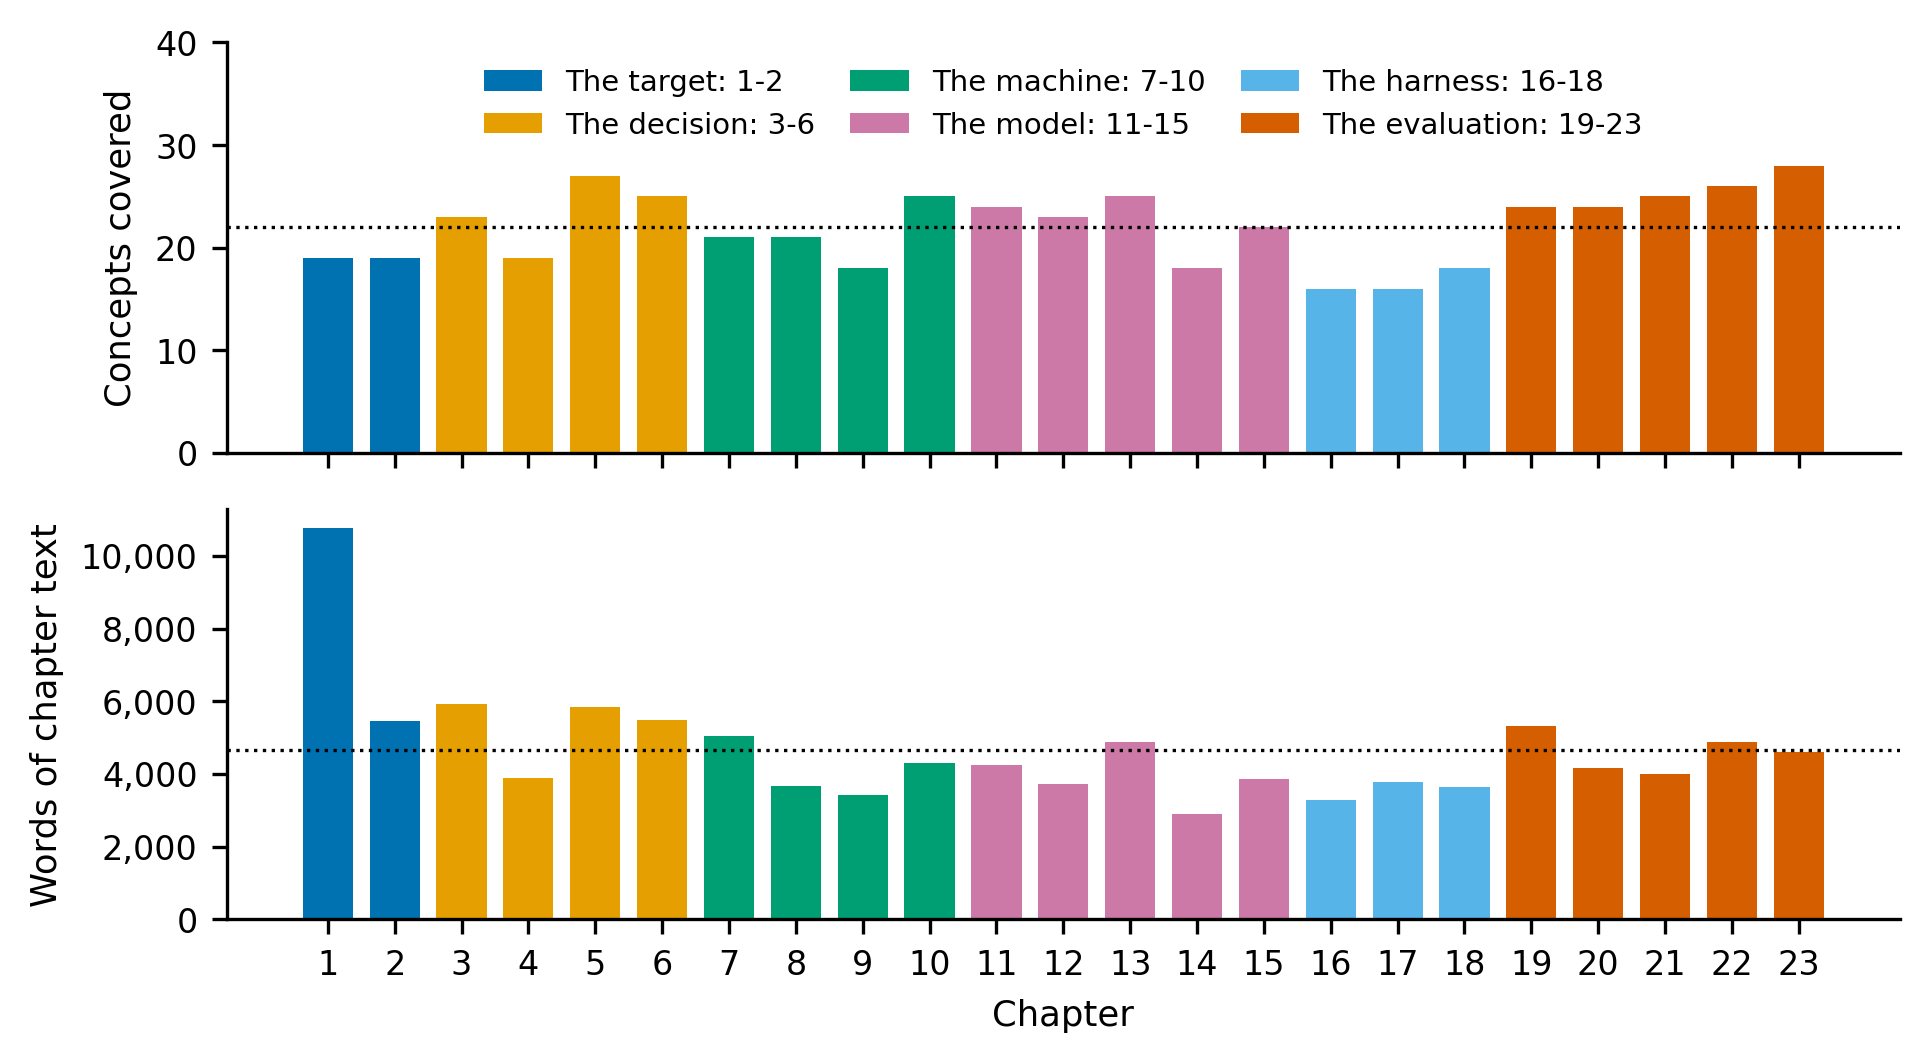
\includegraphics[width=0.95\textwidth]{figures/fig-book-structure.png}
\caption{Concepts covered and words per chapter, colored by part. Words are whitespace-delimited tokens of each chapter's source file, including tables and diagram specifications; the dotted line is the mean. Chapter~1 is long because it also carries the prerequisites, the pipeline overview, and the first worked examples.}
\label{fig:book}
\end{figure}

\subsection{Inventory}

Table~\ref{tab:inventory} counts what the book contains. The 506 concepts are not a list but a graph: 824 dependency edges, 12 foundational concepts with no prerequisite, 193 terminal concepts that nothing else depends on, no isolated node, no cycle, and a longest dependency chain of 16 concepts. Chapters were written in dependency order, so no concept is used before its prerequisites have been introduced. The longest chain runs from \textit{generative AI assistant use} through \textit{small language model} and \textit{repeated runs} to \textit{local, cloud, or hybrid decision}, which is the book's argument in miniature.

\begin{table}[htbp]
\centering
\small
\begin{tabular}{@{}lrl@{}}
\toprule
\textbf{Item} & \textbf{Count} & \textbf{Note} \\
\midrule
Chapters & 23 & about 100,000 words of chapter text \\
Concepts in the learning graph & 506 & 824 dependencies, a directed acyclic graph \\
Glossary terms & 506 & one definition per concept \\
Quiz questions & 230 & ten per chapter, tied to concepts \\
Annotated references & 230 & ten per chapter, each with a relevance note \\
MicroSims & 36 & all at status \textit{built}; none yet \textit{approved} \\
Candidate models & 10 & six with results \\
\bottomrule
\end{tabular}
\caption{What the book contains. ``Built'' means implemented and awaiting review by the author; ``approved'' is reserved for the human author after exercising the controls.}
\label{tab:inventory}
\end{table}

\subsection{Construction by the Pipeline It Evaluates}

The book was generated with the skill chain it benchmarks (Section~\ref{sec:design}): a course description was analyzed and scored, a 506-concept learning graph and taxonomy were generated, chapters were designed from the graph, chapter text was written, and then the glossary, FAQ, quizzes, and references were generated. Each chapter was sized from its own concepts. Every concept carries a Concept Impact Score (CIS): one plus the sum of the CIS of every concept that depends on it, so that a concept many others build on receives a larger word budget. This budget is the same one the conformance score of Section~\ref{sec:measurement} uses to judge generated chapters, so the book's content rules and the benchmark's scorer are one specification applied twice.

The project's agent instructions add rules a generated chapter must satisfy: anti-padding rules that prefer a dense section to a long one, a fixed layout for diagram specifications, and placement rules for the book's learning mascot. We describe them here because they are what the scorer later measures, and because the book is an unusually complete record of how a human author and an AI assistant divided the work: a design-choices page records each decision, who made it, what else was considered, and which choices did not hold up.

\subsection{Status of the Book}

The book is a working draft by an AI assistant under human direction, and it labels its generated content accordingly. The model-results pages are published exactly as each model wrote them, apart from removed links to missing pages, with a banner stating that no person has yet judged them. The MicroSims are implemented but unreviewed. Section~\ref{sec:discussion} returns to what this means for use with learners.

\section{Benchmark Design}
\label{sec:design}

\subsection{The Workload}

The workload is the \textit{ibook-skills} chain \cite{ibookskills}: ten ordered Agent Skills that turn a course description into an intelligent textbook. They validate the course description, generate a learning graph of concepts and dependencies, design the chapter structure, write chapter text, build interactive MicroSims, and generate a glossary, an FAQ, quizzes, and references. The benchmark uses the first three generative skills only, because they carry the structural dependencies that every later stage inherits and because three stages are enough to expose where a local model fails. MicroSims, glossary, FAQ, quizzes, and references are outside this round.

\begin{table}[htbp]
\centering
\small
\begin{tabularx}{\textwidth}{@{}clXl@{}}
\toprule
\textbf{Stage} & \textbf{Skill} & \textbf{Produces; counted as done when} & \textbf{Limit} \\
\midrule
1 & \texttt{learning-graph-generator} & 200 concepts, their dependencies, and a taxonomy, as a CSV file and a JSON file; the run ends on its own and leaves both files & 150 min \\
2 & \texttt{book-chapter-generator} & One directory and outline per chapter, designed from the model's own learning graph & 120 min \\
3 & \texttt{chapter-content-generator} & One run per chapter; a chapter counts as written when its placeholder is gone and it has at least 1,000 words & 90 min per chapter \\
\bottomrule
\end{tabularx}
\caption{The three benchmark stages. Each stage starts from a copy of the previous stage's output. A model stops after two consecutive chapter runs hit the limit.}
\label{tab:stages}
\end{table}

\subsection{The Course and a Reference for Scale}

The course is Algebra~I for high school. Its description is an unchanged copy of the description from a published, cloud-generated Algebra~I textbook \cite{algebra1}. That published book is a reference for scale and not a baseline: it has 200 concepts and 277 dependencies, 13 chapters of about 55,000 words, 13 quizzes, 48 MicroSims, a 197-term glossary, and an 82-question FAQ. It was generated with cloud models and earlier versions of the skills, and no token counts or timings were recorded for it. Every model starts from the same template workspace and the same prompt for each stage. Each prompt is what a person would type to start the skill plus a standing answer to the skill's approval questions, because nobody is present during a run and a paused run measures nothing.

\subsection{Roles}

The design separates three roles that are easy to confuse (Figure~\ref{fig:architecture}).

\begin{itemize}
\item The \textbf{orchestrator} is a cloud-model agent session on the author's laptop. It starts runs, watches them, retrieves output, and runs the scoring programs. It writes no benchmark content.
\item The \textbf{harness} is Claude Code, pinned to one version, run headless in a Docker container on the DGX. It loads a skill, sends prompts to the model, and executes the tools the model requests. The container mounts the skills read-only and exposes only the run directory and its own transcript folder as writable; permission prompts are bypassed inside it because the container is the boundary.
\item The \textbf{model} is an open-weight model served by Ollama on the same machine, bound to the loopback interface. It generates every token of the textbook. The harness is given a placeholder credential and its optional network features are switched off.
\end{itemize}

The rule that follows is simple and was set by the author: \textit{no cloud model may write benchmark content}. The orchestrator may start, observe, and score a run. It may not repair one.

\begin{figure}[htbp]
\centering
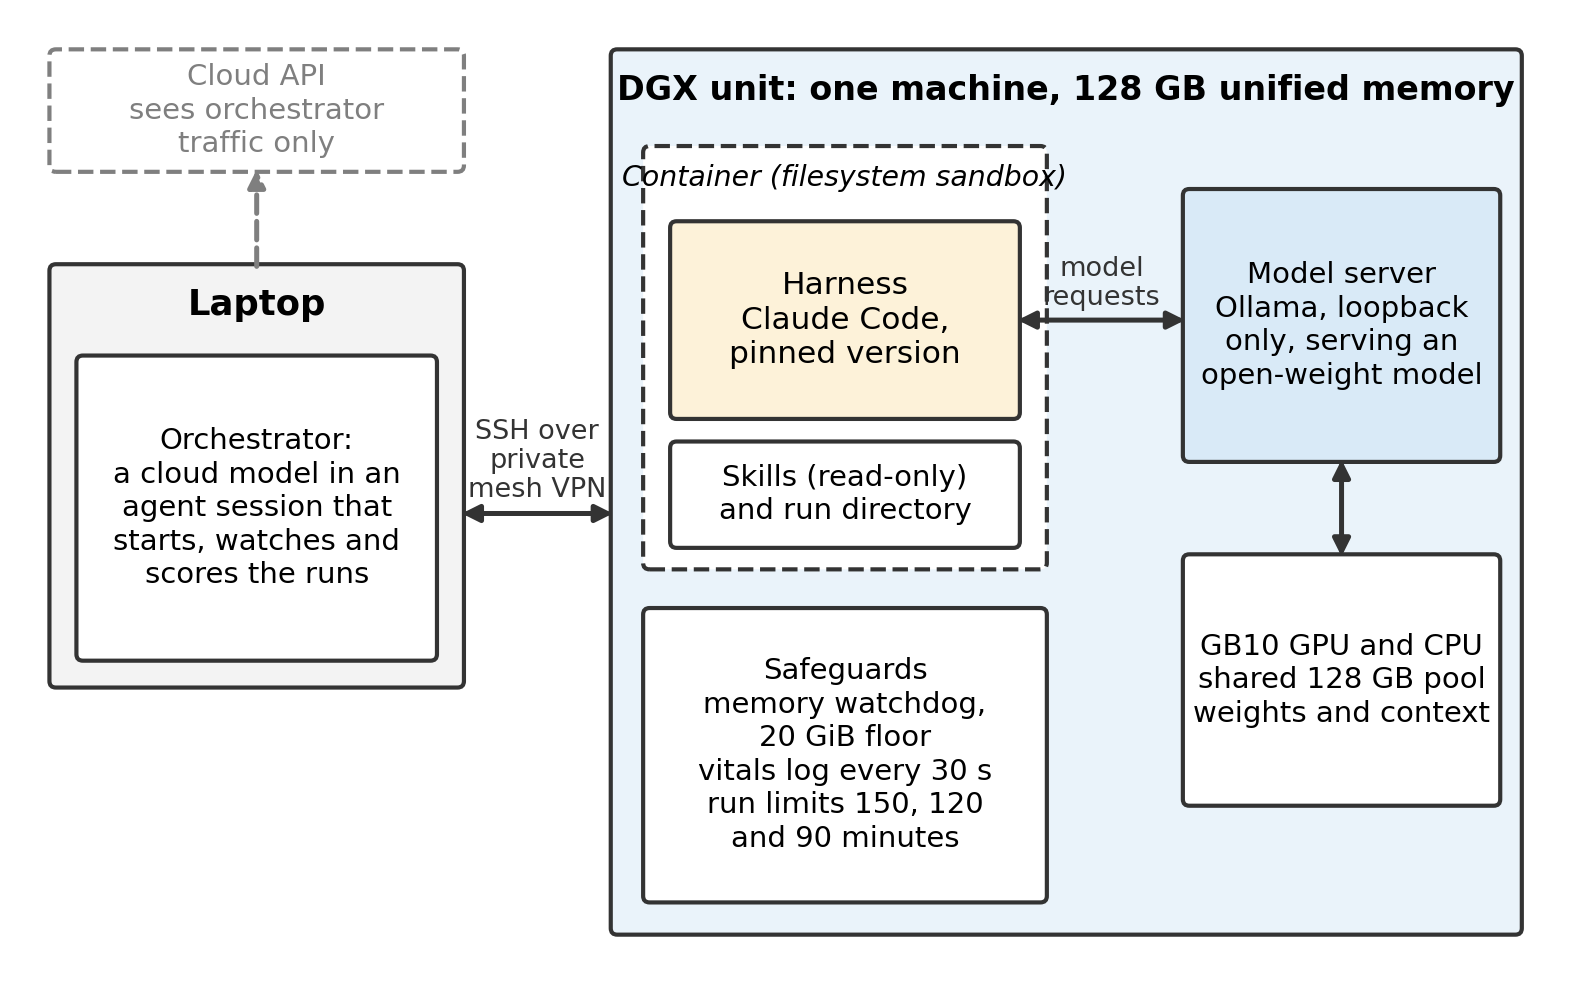
\includegraphics[width=0.85\textwidth]{figures/fig-architecture.png}
\caption{Evaluation architecture. Generation traffic (prompts and tokens) stays on the DGX; the orchestrator's supervision traffic does not. The container is a filesystem sandbox, not a network sandbox, because it shares the host network to reach the model server. No address, host name, or login appears in this paper.}
\label{fig:architecture}
\end{figure}

\subsection{Hardware and Software}

The machines are two identical NVIDIA DGX Spark-class units administered by a third party, reached from the laptop over a private mesh VPN built on WireGuard \cite{donenfeld2017wireguard, pennarun2020tailscale}. All results reported here came from one unit. Table~\ref{tab:hardware} lists the configuration.

\begin{table}[htbp]
\centering
\small
\begin{tabular}{@{}lp{12cm}@{}}
\toprule
\textbf{Component} & \textbf{Value} \\
\midrule
CPU & 20 Arm cores (10 Cortex-X925, 10 Cortex-A725) \\
GPU & NVIDIA GB10 Blackwell, 6,144 CUDA cores \\
Memory & 128~GB LPDDR5x unified, shared by CPU and GPU; 273~GB/s as published by the vendor \cite{nvidia2025dgxspark} \\
Storage & 1~TB NVMe \\
Model server & Ollama, one pinned release, installed in user space, loopback only \\
Harness & Claude Code, one pinned version, in a non-root container \\
Quantization & each publisher's default 4-bit file \\
\bottomrule
\end{tabular}
\caption{Configuration of the unit that produced every result. The GPU has no memory of its own: weights and conversation context compete for the same 128~GB as the operating system and every other program.}
\label{tab:hardware}
\end{table}

\subsection{Candidate Models}

Ten open-weight models were chosen for one 128~GB unit, in the order shown in Table~\ref{tab:models}, \textit{before} any results. The criteria came from the workload: tool calling, a context window of at least 64,000 tokens, a fit in memory with room for that context, and a publisher and license that could be identified. The order put models with early results first and then the models whose publishers' claims came closest to the two abilities the benchmark exercises. Publisher claims come from each model's library page as of October 2026 and were not checked.

\begin{table}[htbp]
\centering
\footnotesize
\begin{tabular}{@{}lrrrrl@{}}
\toprule
\textbf{Model} & \textbf{Params (B)} & \textbf{Active (B)} & \textbf{Disk (GB)} & \textbf{Window (K)} & \textbf{Decode (tok/s)} \\
\midrule
\Qeight & 27 & --- & 17 & 256 & 26$^\dagger$ \\
\Gthirtyone & 30.7 & dense & 20 & 256 & 28--40 \\
\Muse & 30 & --- & 18 & 128 & 13 \\
\Qsix & 35 & $\approx$3 & 22 & 256 & 83--105 \\
\Gtwentysix & 25.2 & 3.8 & 18 & 256 & 86--130 \\
\Nemo & 30 & 3 & 25 & 1,000 & 84--105 \\
\Mistral & 128 & dense & 80 & 256 & 3 \\
\Gptoss & 117 & 5.1 & 65 & 128 & 38--44 \\
\Devstral & 24 & --- & 15 & 384 & 15 \\
\Granite & $\approx$30 & dense & 17 & 128 & 12 \\
\bottomrule
\end{tabular}
\caption{The ten candidates. Parameters, active parameters per token, download size, and declared context window are as stated by each publisher. Decode speed is from the model-only tests with reasoning off, except $^\dagger$, which is the speed on the longest turn of that model's stage~1 harness run. A dash means the publisher's page does not state an active count. Licenses are Apache~2.0 for seven models (for \Qeight, as reported by secondary sources and not verified), a modified MIT license for \Mistral, and unstated on the library page for \Qsix{} and \Nemo.}
\label{tab:models}
\end{table}

\subsection{Protocol}

Each stage run starts from a fresh copy of its input, so no run can alter the input of another. The runner records a status file (exit code and wall-clock seconds), the full event stream, and a final result with turn and token counts. Stage 3 runs once per chapter, carrying the book written so far into each run, with a 90-minute limit per chapter and a cap of 150 turns. The server's context length was set for each model to the largest value that a linear estimate said would leave 45~GiB of memory free: 163,840 tokens for eight models and 131,072 for \Gptoss. Reasoning, where a model supports it, was left at the model's default in the harness. Sampling parameters were the server and model defaults. A memory watchdog (floor 20~GiB, GPU temperature ceiling) killed harness containers and unloaded the model before a unified-memory machine could freeze, and a vitals log recorded memory, temperature, power, and load every 30 seconds so that a freeze would leave evidence behind.

\subsection{Two Layers of Testing}

Models were tested alone before they were tested in the harness. The model-only test runs five short tasks through the server's API with no harness: Markdown writing under format rules, p5.js code, schema-constrained JSON, a tool call, and a 30,000-token prompt with a fact to retrieve. A model that cannot keep a blank line before a list fails in seconds and not after an hour. The second layer is a three-minute harness smoke test, in which the model runs the course-description-analyzer skill and the build is checked, followed by the three benchmark stages. The layers have different failure modes, which Section~\ref{sec:discussion} returns to: a model can pass the first and fail the second.

\subsection{Controlled and Uncontrolled Variables}

The independent variable is the model. Table~\ref{tab:controls} records what was held fixed and what was not. A controlled variable is a claim that must be defensible, so the table also records the ones that were not kept.

\begin{table}[htbp]
\centering
\small
\begin{tabularx}{\textwidth}{@{}lXl@{}}
\toprule
\textbf{Variable} & \textbf{How it was handled} & \textbf{Status} \\
\midrule
Course, prompts & One unchanged course description; one prompt file per stage & Controlled \\
Harness, server & Pinned Claude Code version; pinned Ollama release & Controlled \\
Skills & One checkout, read-only; a faulty example in one skill corrected before the comparison runs & Controlled \\
Hardware & One unit for all results & Controlled \\
Starting state & Fresh copy of the input for every run & Controlled \\
Time limits & 150, 120, and 90 minutes; two consecutive chapter timeouts end a model's stage~3 & Controlled \\
Quantization & Each publisher's default 4-bit file & Controlled, but differs by publisher \\
Context length & Largest that keeps 45~GiB free, per model & Uncontrolled \\
Reasoning mode & Model default in the harness; off in the model-only tests & Uncontrolled \\
Sampling & Server and model defaults & Uncontrolled \\
Server behavior & One server re-read the whole conversation on every turn; cause not found & Uncontrolled \\
Run-to-run variance & One run per model per stage & Not measured \\
Supervision & A cloud orchestrator read run output to monitor and score & Uncontrolled \\
\bottomrule
\end{tabularx}
\caption{Controlled and uncontrolled variables.}
\label{tab:controls}
\end{table}

One attempt did not follow the protocol. The first stage~1 attempt for \Gthirtyone{} ran on the second unit at a 256,000-token context and was lost when that machine stopped responding; the result reported here is the second attempt, on the first unit at 163,840 tokens. The second unit stopped responding twice, both times minutes into a run of the same model. The administrator found no recorded out-of-memory kill, GPU error, kernel panic, or thermal shutdown and reported intermittent loss of power to that unit. The cause is not established, and no result from that unit is used.

\section{Measuring What Was Produced}
\label{sec:measurement}

Two kinds of measurement are used. \textit{Structural checks} ask whether an output exists and is well formed, which a program can verify exactly. The \textit{chapter-conformance score} asks how closely a written chapter follows the book's content rules. Neither judges whether the mathematics is correct or the explanation is good; that remains a human review that has not yet been done.

\subsection{Structural Checks}

For stage~1 the checks are: every expected file is present; the CSV has the required columns; the concept count matches the target of 200; identifiers are consecutive from~1; no label is duplicated; no label exceeds 32 characters; every dependency refers to an existing concept; no concept lies on a cycle; the JSON file agrees with the CSV; and a strict site build succeeds. The report also counts concepts with no prerequisite and concepts connected to nothing. For stages~2 and~3 the checks are: chapter files exist, concepts are assigned to chapters, words per chapter, and whether the placeholder text is gone. A chapter is \textit{written} when its placeholder is gone and it has at least 1,000 words.

\subsection{The Chapter-Conformance Score}

The author set four requirements: use objective measurements; include adherence to the book's content rules, the placement of diagrams, and the quality of their specifications; report word count, diagram count, and reading level for each chapter; and favor consistent quality over high absolute quality. Three further constraints follow from how the benchmark runs. The same files must always receive the same score; the program must run on a DGX with nothing beyond the Python standard library; and every number must be explainable, so that a chapter that scores badly shows which rule it broke.

\paragraph{Budget from the chapter's own concepts.}
Each concept $c$ has a Concept Impact Score $\mathrm{CIS}(c)$, one plus the sum of $\mathrm{CIS}$ over every concept that depends on it. Its normalized importance is
\begin{equation}
E(c) = \frac{\ln\bigl(\mathrm{CIS}(c)+1\bigr)}{\ln\bigl(\mathrm{CIS}_{\max}+1\bigr)},
\end{equation}
and $E(c)$ assigns a tier (Table~\ref{tab:tiers}). A chapter's word budget is the sum of its concepts' targets. A chapter of mostly Tier~A concepts is therefore expected to run several times longer than one of mostly Tier~C, and the score does not normalize that variation away. The word-fit sub-score is a plateau: zero below 20\% of the low target, full credit from 60\% of the low target to 125\% of the high target, and falling to zero at 250\% of the high target. A chapter is never rewarded for exceeding its budget, because the content guide says a dense chapter beats a padded one.

\begin{table}[htbp]
\centering
\small
\begin{tabular}{@{}clrl@{}}
\toprule
\textbf{Tier} & \textbf{$E(c)$} & \textbf{Target words} & \textbf{Required elements} \\
\midrule
A & $\ge 0.5$ & 500--750 & worked example, plus a diagram, chart, table, or MicroSim \\
B & 0.2 to 0.5 & 250--400 & worked example \\
C & $<0.2$ & 120--200 & a clear definition \\
\bottomrule
\end{tabular}
\caption{Concept tiers and per-concept word targets taken from the book's content-generation guide.}
\label{tab:tiers}
\end{table}

\paragraph{Six dimensions.}
Each dimension is a weighted mean of sub-scores in $[0,1]$. A sub-score that does not apply to a chapter is dropped and the remaining weights are rescaled, so a chapter with no admonitions is not penalized for their absence. The chapter score is $Q = 100\sum_d w_d s_d \big/ \sum_d w_d$ with the weights in Table~\ref{tab:dimensions}, which were set by hand because no human ratings exist yet.

\begin{table}[htbp]
\centering
\small
\begin{tabularx}{\textwidth}{@{}lrX@{}}
\toprule
\textbf{Dimension} & \textbf{Weight} & \textbf{Question it asks} \\
\midrule
Budget & 20 & Does the chapter hold the words, worked examples, and non-text elements that its own concepts call for, and cover the concepts it lists? \\
Diagram placement & 20 & Is each diagram introduced by prose, defined before it appears, near the text it illustrates, and spread through the chapter? \\
Diagram specification & 20 & Does each specification carry the 18 required fields at the precision that 14 written rules ask for? \\
Format & 15 & Does the Markdown render, and are headings, admonitions, and mascot used as the guide says? \\
Padding & 10 & Does the chapter repeat itself or pad with filler (duplicate sentences, windowed compression ratio, stock phrases, templated specifications)? \\
Reader fit & 15 & Is the reading level right for the audience, with equations and worked examples present? \\
\bottomrule
\end{tabularx}
\caption{The six dimensions of the chapter score and their weights.}
\label{tab:dimensions}
\end{table}

Three design choices deserve explanation. First, the specification dimension encodes the rules of the chapter-content skill itself, so a diagram counts as correctly placed when the skill's own batch tool will find and build it, even if a stricter reading of the rules would disagree; a score should agree with the toolchain that consumes the output. Second, reading grade is the Flesch--Kincaid grade \cite{kincaid1975} of the prose with math, code, tables, and specifications removed, against a target of 9.0 for Algebra~I. Third, equations are \textit{counted but not scored}: each chapter and book reports how many equations are well formed and how many the site would display as source text. The count is a syntax check, written from the KaTeX function list and not by running KaTeX, and it is kept out of the score so that every number in this paper holds the value at which the weights were checked.

\paragraph{From chapters to a book.}
Algorithm~\ref{alg:book} gives the book score. The book's composite score is its level multiplied by its consistency, where consistency is one minus the coefficient of variation of the written chapters. Unwritten chapters enter the level as zero and are left out of the consistency, so that one fact, that a chapter is missing, is not charged twice.

\begin{algorithm}[htbp]
\caption{Scoring one generated book}
\label{alg:book}
\begin{algorithmic}[1]
\Require chapters $c_1,\dots,c_N$ with their concept tables; the book's learning graph
\For{each chapter $c_i$}
  \If{$c_i$ holds the placeholder text or has fewer than 1,000 words}
    \State $Q_i \gets 0$ \Comment{stub}
  \Else
    \State compute the word budget $[L_i,H_i]$ from the tiers of $c_i$'s concepts
    \State score the six dimensions $s_d\in[0,1]$, dropping sub-scores that do not apply
    \State $Q_i \gets 100\sum_d w_d s_d \big/ \sum_d w_d$
  \EndIf
\EndFor
\State $\mathrm{level} \gets \frac{1}{N}\sum_{i} Q_i$ \Comment{stubs count as 0}
\State $\mu,\sigma \gets$ mean and standard deviation of $Q_i$ over \emph{written} chapters only
\State $\mathrm{consistency} \gets 100\,(1-\sigma/\mu)$ \Comment{undefined for fewer than two written chapters}
\State \Return $\mathrm{level}\times\mathrm{consistency}/100$
\end{algorithmic}
\end{algorithm}

Several ways of favoring consistency were weighed. The mean alone ignores spread, and a book of ten excellent chapters and ten stubs would tie a book of twenty middling ones. A mean with a variance penalty trades points for spread at an invented exchange rate. The lowest chapter alone lets one bad chapter in twenty decide the whole book. The geometric mean of level and consistency is too generous to a uniformly poor book: level 20 at consistency 95 scores 44, where the product scores 19. The product keeps a uniformly poor book poor and cuts a lopsided one by its spread.

\subsection{Why Counts and Not a Language Model}

A model asked to rate a chapter would be quicker to build and would notice what a regular expression cannot, such as an explanation that is wrong. It would also give a different answer on each run, bring its own bias toward text that sounds like itself \cite{zheng2023judge, panickssery2024selfpref}, and, if hosted in the cloud, send the generated books to a third party. The rules to be checked are written, specific, and mostly countable, so a program can check them, repeat itself exactly, and run on the DGX. The cost is real: a counting score can be satisfied by text that has the right fields and nothing in them. We do not claim otherwise.

\subsection{Validation and Its Limits}

The checks we ran on the score are modest, and we report them with the bugs they missed.

\begin{itemize}
\item \textbf{Determinism.} The same input scored twice gave identical output.
\item \textbf{Insensitivity to size.} Across the 49 written chapters, the Spearman correlation of the chapter score with body words is $-0.10$, with the number of diagram specifications $0.15$, and with the number of equations $0.15$. The score does not track size, which is what the plateau and the saturating sub-scores were built to achieve.
\item \textbf{Reweighting.} We multiplied each of the six dimension weights by an independent uniform draw from $[0.6,1.4]$, 500 times, and recomputed the composite scores (Section~\ref{sec:quality}).
\item \textbf{Bugs that survived.} Three defects passed the checks above and were found later: a header rule stricter than the skill's own parser, a function that treated a whole chapter as boilerplate, and a case-insensitive pattern that matched an HTML tag and failed 278 of 282 specification blocks. None showed in the totals. Two were found by reading single chapters whose sub-scores looked wrong, and the third by tabulating how often each check failed: a check that fails 99\% of the time is a defect. One chapter had been scored about 14 points too low.
\end{itemize}

Three limits remain. The thresholds, such as the compression ratio and words per sentence, were read off the same six books they now score, so they fit this corpus and must be revisited for a new course or model. The weights are the author's and the assistant's opinions, untested against a human. And the specification checks encode one version of one skill, so a new skill version can make a check wrong without any change in the chapters.

\section{Results}
\label{sec:results}

Every number in this section comes from one run per model per stage on one unit. They support statements about what happened in those runs; they do not rank the models in general.

\subsection{Before the Benchmark: Model-Only and Smoke Tests}

The model-only tests and the harness smoke test eliminated or flagged several candidates before stage~1, and they did not predict everything. \Mistral{} loaded and ran at 3 tokens per second, and with the weights resident it used 88~GiB at a 32,000-token context, so no context of 64,000 tokens or more fits beside it; it was not run in the harness. \Muse{} returned invalid JSON on the schema task and ran at 13 tokens per second. \Gptoss{} returned the wrong value from the long prompt three times, and in one of two smoke runs wrote a tool call as plain text and stopped after one turn. \Gthirtyone{} passed every format rule in the model-only tests, twice, and \Qeight{} followed every rule as well. \Gtwentysix{} twice broke two rules (a blank line before a list, and a p5.js call that fails when run), and \Nemo{} broke four. These results shaped expectations and did not decide the outcome: as Section~\ref{sec:discussion} shows, a model that follows every rule in isolation can still fail in the harness.

\subsection{Stage 1: Learning Graph}

Six of the ten models produced a learning graph. Table~\ref{tab:stage1} gives the structural result. All six graphs were acyclic and every JSON file matched its CSV. None of these checks says that the concepts are the right ones for Algebra~I or that the dependencies make sense; that judgment has not been made.

\begin{table}[htbp]
\centering
\footnotesize
{\setlength{\tabcolsep}{4pt}\begin{tabular}{@{}p{3.0cm}rrrrrp{4.7cm}@{}}
\toprule
\textbf{Model} & \textbf{Min.} & \textbf{Concepts} & \textbf{Deps} & \textbf{Calls (failed)} & \textbf{Peak (K)} & \textbf{Notable defects} \\
\midrule
\Qeight & 102 & 200 & 299 & 55 (1) & 108 & none structural \\
\Gthirtyone & 21 & 200 & 348 & 50 (8) & 68 & taxonomy page missing; navigation not updated \\
\Qsix & 22 & 200 & 273 & 55 (4) & 135 & 19 concepts with no prerequisite; 1 duplicate label \\
\Nemo & 18 & 199 & 494 & 140 (7) & 147 & one concept short; navigation not updated \\
\Gtwentysix & 6 & 200 & 483 & 51 (5) & 60 & 40 duplicate labels; index page missing; navigation not updated \\
\Gptoss & 17 & 200 & 180 & 28 (0) & 50 & 19 concepts connected to nothing \\
\midrule
\Granite & 150$^{\dagger}$ & --- & --- & 32 (4) & 50 & reached only the concept list \\
\Muse & 6 & --- & --- & 6 (0) & 125 & lost the task after a few steps \\
\Devstral & $<$1 & --- & --- & 0 & 21 & first tool call written as text \\
\Mistral & --- & --- & --- & --- & --- & not run: no usable context fits \\
\bottomrule
\end{tabular}}
\caption{Stage~1 results. Min.\ is wall-clock minutes; $^{\dagger}$ stopped at the 150-minute limit. ``Peak'' is the largest conversation, in thousands of tokens, that the server logged for that model. Calls are tool calls, with the number that failed in parentheses.}
\label{tab:stage1}
\end{table}

Two observations stand out. First, speed spans a factor of about 18: from 6 to 102 minutes for the same task, and from 6.7 to 111 seconds of wall-clock per tool call. The slowest model, \Qeight, produced the cleanest graph: exactly 200 concepts and 299 dependencies, two concepts with no prerequisite, no duplicate or overlong label, and a site that builds. Second, the models that produced a graph made between 28 and 140 tool calls. \Nemo{} needed 140, nearly three times as many as any other, and its conversation grew to 147,000 tokens.

\subsection{Stages 2 and 3: Chapter Structure and Chapter Text}

All six models that produced a graph completed stage~2 and designed between 10 and 14 chapters. Stage~3 is where they diverged (Figure~\ref{fig:completion}, Table~\ref{tab:stage3}). Two models, \Nemo{} and \Qsix, wrote every chapter they had designed. The other four stopped short, and \Qeight{} was too slow to write one.

\begin{figure}[htbp]
\centering
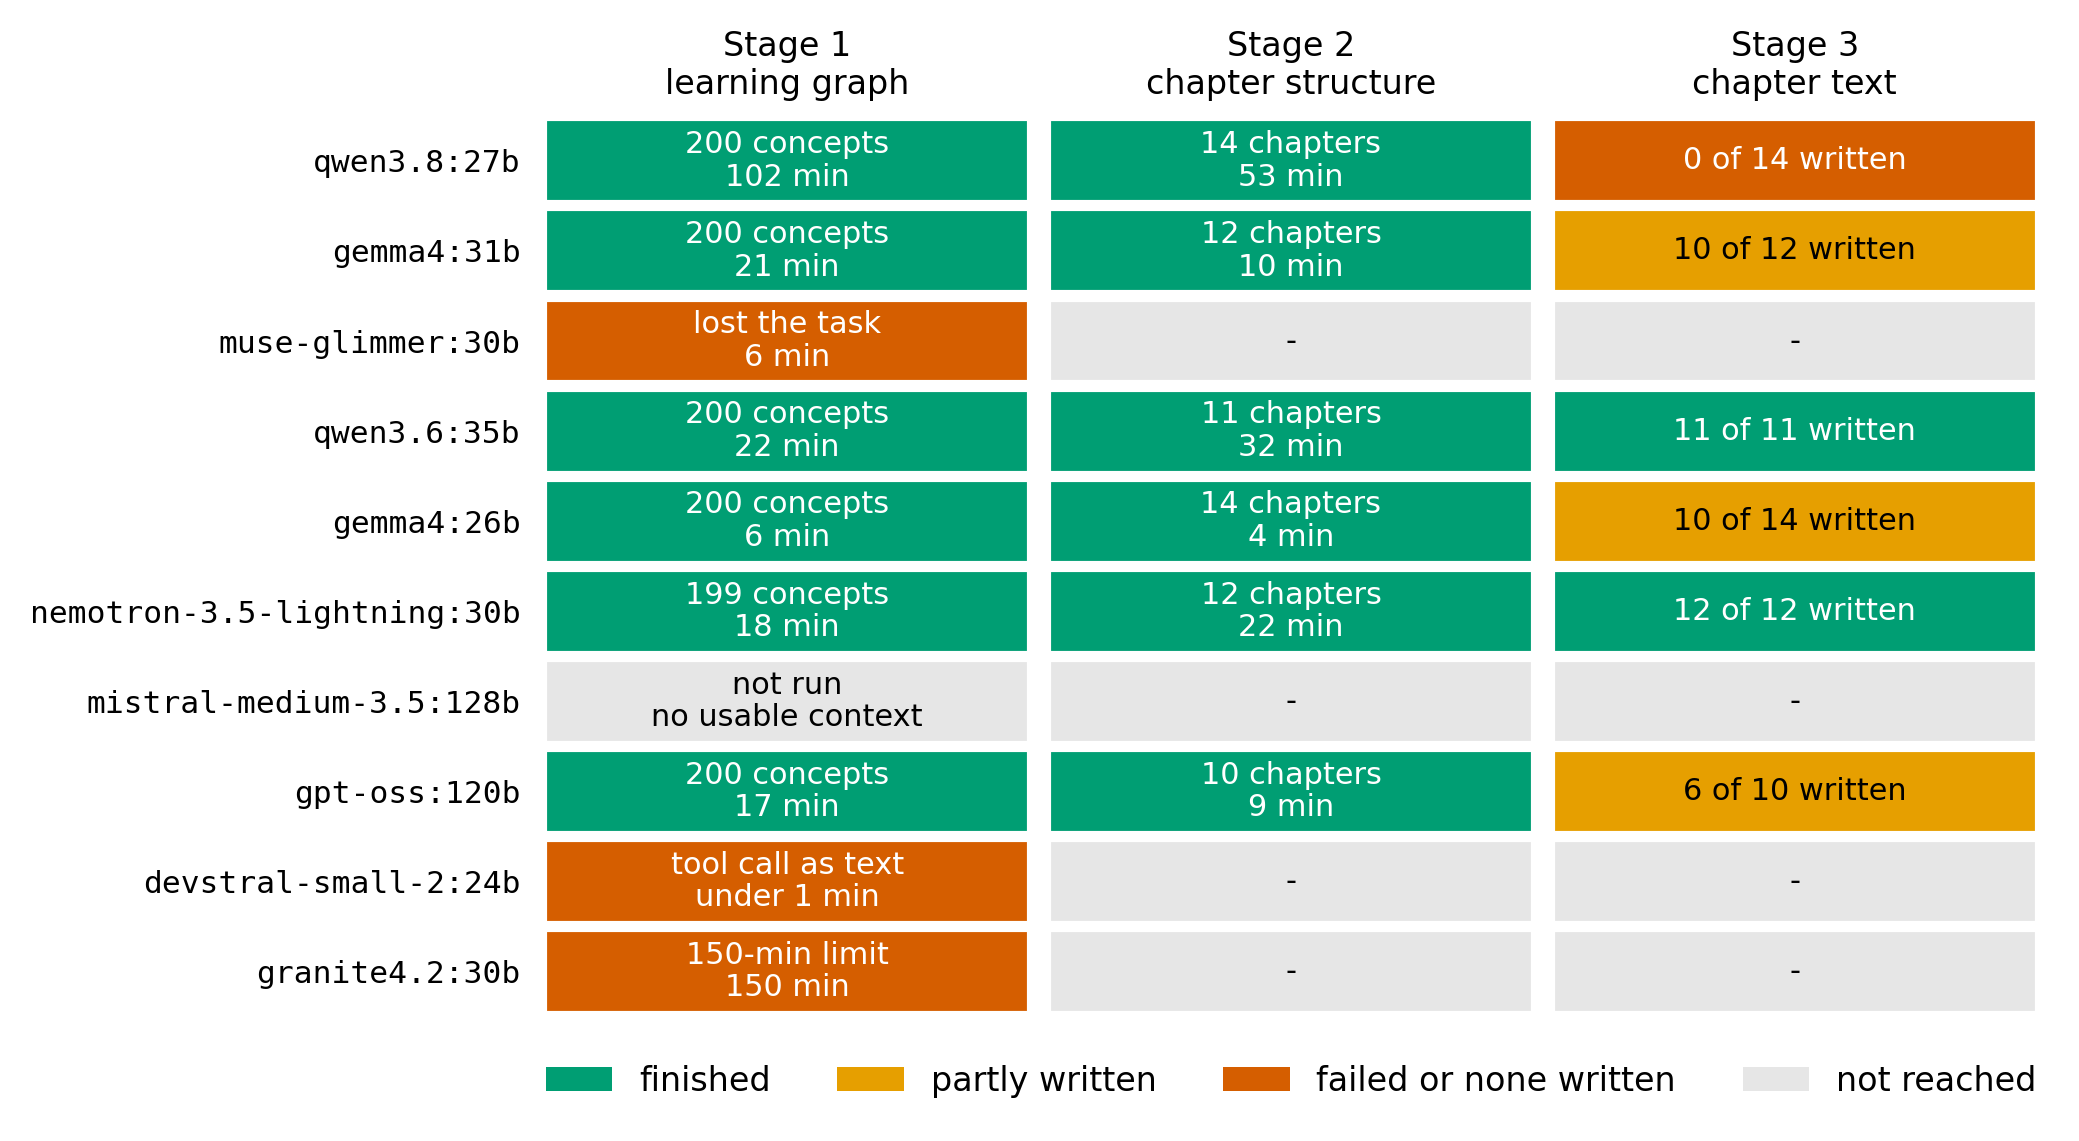
\includegraphics[width=0.95\textwidth]{figures/fig-completion.png}
\caption{How far each of the ten candidates got. Models are in the order in which they were chosen for testing, before any results. Cell text gives concept or chapter counts and wall-clock minutes for the one run.}
\label{fig:completion}
\end{figure}

\begin{table}[htbp]
\centering
\small
\begin{tabularx}{\textwidth}{@{}lrrrrX@{}}
\toprule
\textbf{Model} & \textbf{Designed} & \textbf{Stage 2} & \textbf{Written} & \textbf{Stage 3} & \textbf{Chapters not written} \\
\midrule
\Nemo & 12 & 22 min & 12 & 2.0 h & --- \\
\Qsix & 11 & 32 min & 11 & 1.3 h & --- \\
\Gthirtyone & 12 & 10 min & 10 & 4.3 h & 1 stopped at the 90-min limit; 1 ended on a stray control token \\
\Gtwentysix & 14 & 4 min & 10 & 1.7 h & 3 halted by the skill's own prerequisite check; 1 ended without writing \\
\Gptoss & 10 & 9 min & 6 & 1.5 h & 4 announced the skill, then ended the turn \\
\Qeight & 14 & 53 min & 0 & 3.0 h & 2 stopped at the limit; 12 not run \\
\bottomrule
\end{tabularx}
\caption{Stages~2 and~3. ``Designed'' is the number of chapters the model's own stage~2 output defined. Stage~3 time is the sum of the chapter runs.}
\label{tab:stage3}
\end{table}

\subsubsection{Failure Taxonomy}

The unfinished runs fail in a small number of recognizable ways (Table~\ref{tab:failures}). Most are failures of protocol or persistence and not of prose: the model did not produce a well-formed tool call, announced work instead of doing it, ran out of time, or lost the task as its conversation grew.

\begin{table}[htbp]
\centering
\footnotesize
\begin{tabular}{@{}p{2.7cm}p{7.0cm}p{4.6cm}@{}}
\toprule
\textbf{Failure} & \textbf{What was observed} & \textbf{Where} \\
\midrule
Tool call written as text & The first call appears as plain text; the harness sees no call and the run ends after one turn & \Devstral{} (both harness tests); \Gptoss{} (one smoke run) \\
Announces, does not act & The model says the skill is running, as if something else will do the work, and ends its turn without writing the chapter & \Gptoss: 4 of 10 chapters \\
Stray control token & The model's whole reply is a control token, not a tool call; the run ends after four turns & \Gthirtyone: 1 chapter \\
Ends without output & The run ends having written nothing & \Gtwentysix: 1 chapter \\
Self-inflicted precondition halt & The skill's own check finds that the chapter depends on concepts placed in later chapters, and the model stops as the skill requires; the cause is the model's own stage~2 design & \Gtwentysix: 3 chapters \\
Time limit & About twenty tool calls in 90 minutes without reaching the step that writes the file; or 150 minutes with only the concept list written & \Qeight: 2 chapters; \Granite{} (stage~1); \Gthirtyone: 1 chapter \\
Lost the task & The first prompt is 35,000 tokens against 17,000 to 21,000 for other models; within eight turns the conversation is at 120,000 tokens, the edge of its window, and the model answers with a greeting & \Muse \\
No usable context & The weights leave too little memory for a context of useful length & \Mistral \\
\bottomrule
\end{tabular}
\caption{Failure classes observed, with where each occurred.}
\label{tab:failures}
\end{table}

\subsection{Time and Effort}

Table~\ref{tab:effort} and Figure~\ref{fig:time} give machine time for the three stages. The fastest complete-or-partial books took 1.8 to 2.7 hours. \Gthirtyone{} took 4.8 hours, of which 1.5 hours was one chapter run that reached the 90-minute limit; excluding it, 3.3 hours. \Qeight{} spent 5.6 hours, 3.0 of them on two chapter runs that wrote nothing.

\begin{figure}[htbp]
\centering
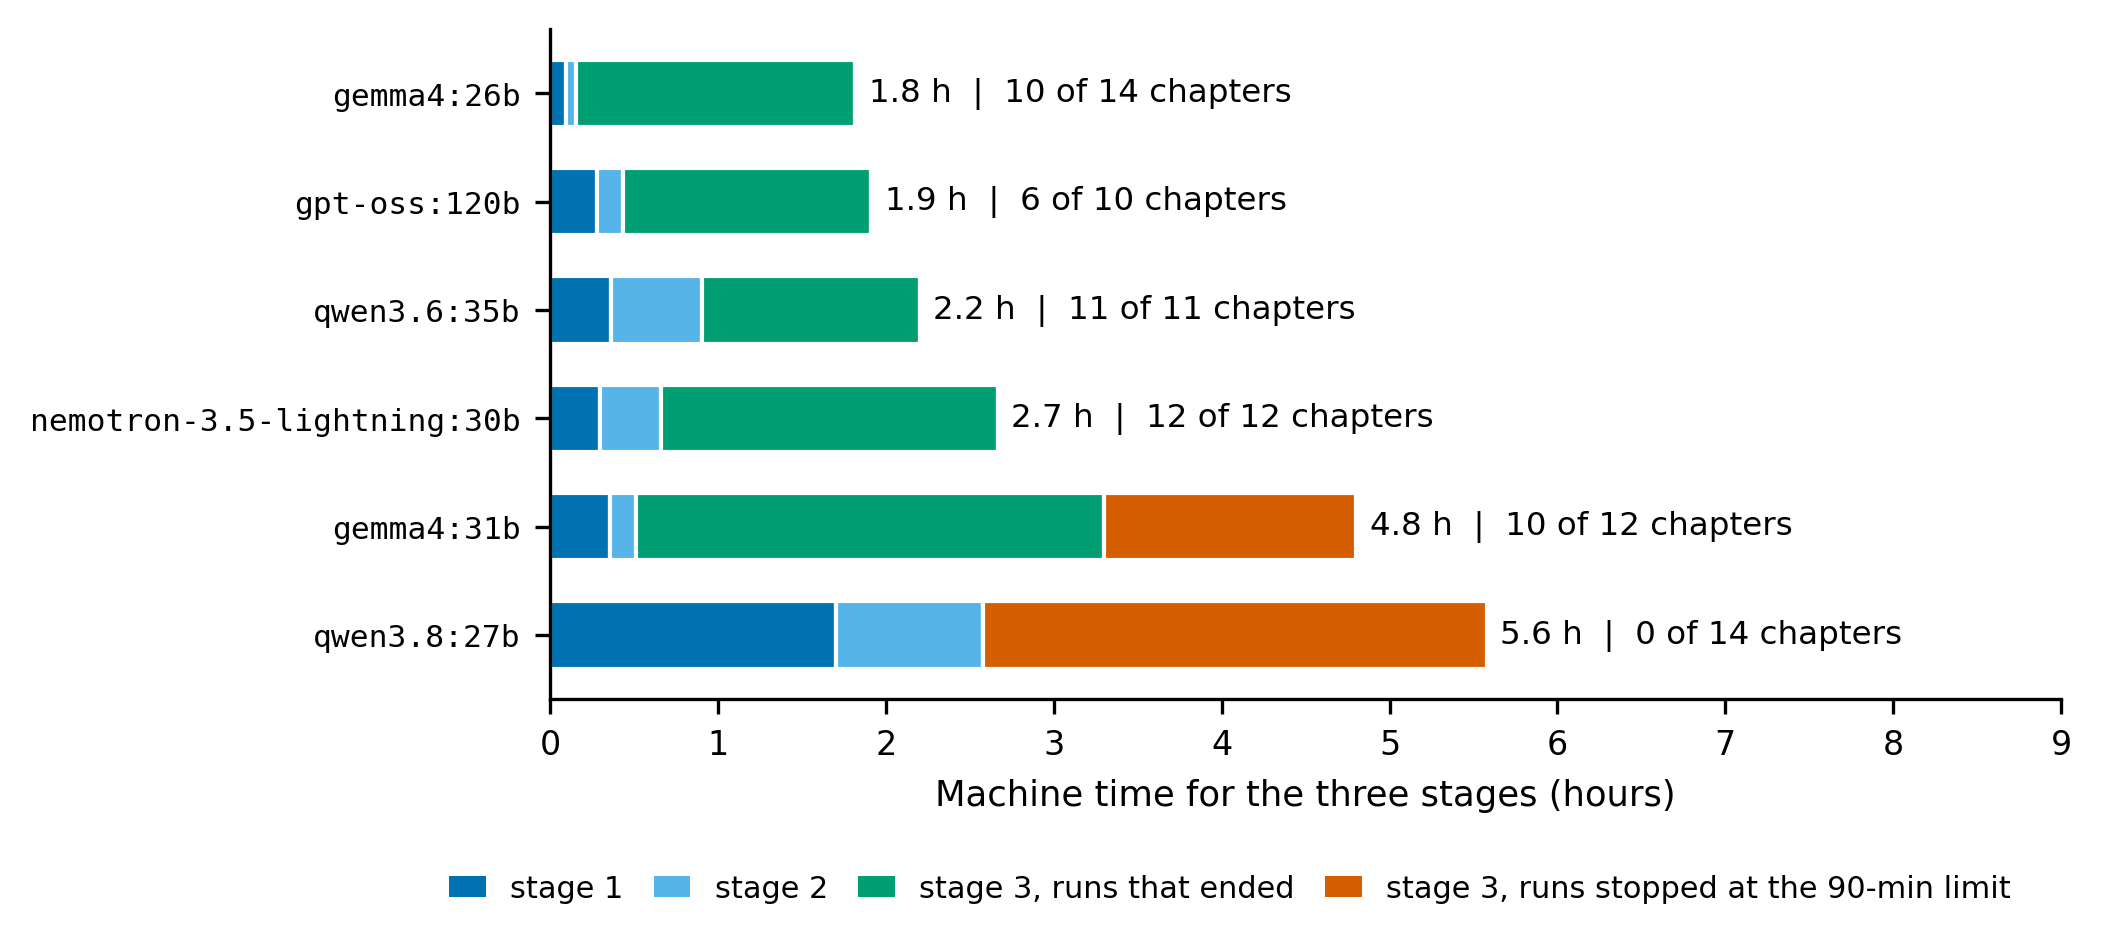
\includegraphics[width=0.95\textwidth]{figures/fig-time.png}
\caption{Machine time for the three stages, by stage, for the six models that produced a graph. Red segments are chapter runs stopped at the 90-minute limit.}
\label{fig:time}
\end{figure}

\begin{table}[htbp]
\centering
\small
{\setlength{\tabcolsep}{5pt}\begin{tabular}{@{}lrrrrr@{}}
\toprule
\textbf{Model} & \textbf{Hours} & \textbf{Calls} & \textbf{Failed} & \textbf{Tokens (K)} & \textbf{Median chapter (min)} \\
\midrule
\Gtwentysix & 1.8 & 416 & 38 (9\%) & 303 & 7.4 \\
\Gptoss & 1.9 & 158 & 7 (4\%) & 108 & 10.1 \\
\Qsix & 2.2 & 465 & 33 (7\%) & 437 & 6.4 \\
\Nemo & 2.7 & 691 & 77 (11\%) & 532 & 8.3 \\
\Gthirtyone & 4.8 & 265 & 52 (20\%) & 171$^{*}$ & 14.1 \\
\Qeight & 5.6 & 128 & 2 (2\%) & 81$^{*}$ & 90 (limit) \\
\bottomrule
\end{tabular}}
\caption{Effort across the three stages. Output tokens are as reported by the server and include reasoning. $^{*}$A run stopped at the limit writes no result record, so its tokens are missing; for \Qeight{} the figure covers stages~1 and~2 only.}
\label{tab:effort}
\end{table}

Three details matter for planning. Tool-call failure rates ranged from 2\% to 20\%, and the model that had passed every format rule in isolation, \Gthirtyone, had the highest rate in the harness. Two models drove the conversation to the configured window: the server logged tasks of 163,832 tokens for \Nemo{} and 163,082 for \Qsix{} against a window of 163,840, so at least one task of each was at or near the limit. And on the server used, one model's per-turn cost was dominated not by generating but by re-reading: for \Qeight, the server restored a checkpoint just past the system prompt and re-read the rest of the conversation on each turn, adding one to two minutes per turn, and one turn spent 19 minutes, nearly all on reasoning. The cause was not identified.

\subsection{Chapter Conformance}
\label{sec:quality}

Table~\ref{tab:quality} gives the conformance scores of the five books with written chapters, and Figure~\ref{fig:quality} shows each chapter.

\begin{table}[htbp]
\centering
\small
{\setlength{\tabcolsep}{4pt}\begin{tabular}{@{}lrrrrrrr@{}}
\toprule
\textbf{Model} & \textbf{Written} & \textbf{Level} & \textbf{Consist.} & \textbf{Floor} & \textbf{Headline} & \textbf{Prose wds} & \textbf{Grade} \\
\midrule
\Qsix & 11 of 11 & 76.4 & 84.1 & 55.9 & \textbf{64.3} & 51,900 & 10.5 \\
\Gthirtyone & 10 of 12 & 69.8 & 91.1 & 68.7 & \textbf{63.6} & 16,137 & 9.4 \\
\Nemo & 12 of 12 & 66.1 & 79.3 & 35.2 & \textbf{52.5} & 52,792 & 11.5 \\
\Gtwentysix & 10 of 14 & 53.4 & 79.1 & 54.5 & \textbf{42.3} & 22,569 & 10.4 \\
\Gptoss & 6 of 10 & 40.9 & 95.3 & 63.5 & \textbf{39.0} & 5,658 & 9.6 \\
\Qeight & 0 of 14 & 0.0 & --- & --- & --- & --- & --- \\
\bottomrule
\end{tabular}}
\caption{Conformance of each book, scored on 49 written chapters. Level is the mean chapter score with stubs as 0; consistency is $100(1-\mathrm{CV})$ over written chapters; floor is the lowest written chapter; headline is level times consistency over 100. Prose words exclude specifications, code, and the concept table. Grade is the mean Flesch--Kincaid grade of the prose against a target of 9.0.}
\label{tab:quality}
\end{table}

\begin{figure}[htbp]
\centering
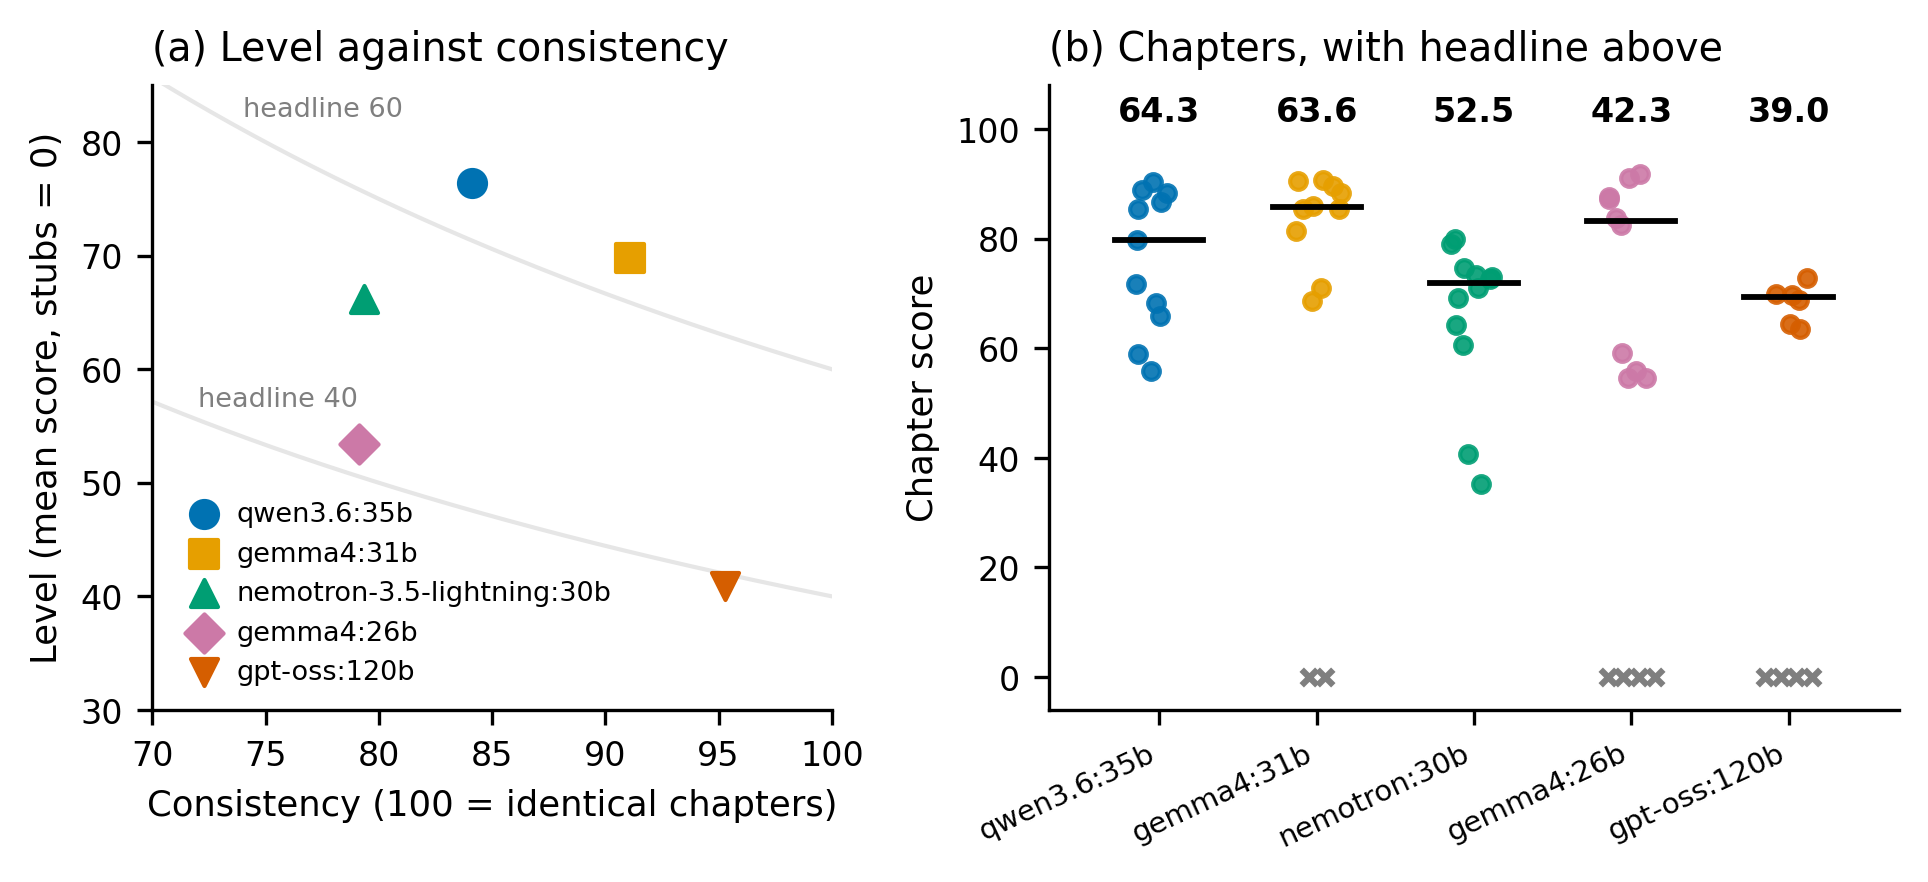
\includegraphics[width=\textwidth]{figures/fig-quality.png}
\caption{(a) Level against consistency; light curves are lines of constant headline. (b) Every chapter score; the bar is each book's median, a gray cross is an unwritten chapter scored 0, and the number above is the headline.}
\label{fig:quality}
\end{figure}

\paragraph{Ordering.}
\Qsix{} and \Gthirtyone{} are within a point of each other on the headline. Reweighting confirms they should be read as a tie: with each dimension weight perturbed by a uniform factor in $[0.6,1.4]$, the full ordering of the five books was unchanged in 61\% of 500 trials, and only two pairs ever swapped: \Qsix{} and \Gthirtyone{} in 39\% of trials, and \Gtwentysix{} and \Gptoss{} in 6\%. Beyond those pairs the order is stable: \Nemo{} stays third.

\paragraph{Level versus consistency.}
The headline separates two things that a mean would blur. \Gptoss{} has the highest consistency of any book, 95.3, because it wrote only six chapters and those six resemble each other; its level is the lowest. \Gthirtyone{} combines high consistency (91.1) with the highest floor (68.7) but lost two chapters. \Nemo{} has the lowest floor, 35.2, from two chapters that it wrote poorly, and the lowest consistency among books that wrote every chapter. This is the behavior the product was chosen to produce.

\paragraph{What the dimensions show.}
Table~\ref{tab:dims} gives the dimension means. Padding is near ceiling for every book (91 to 100), which is why its weight was lowered from 15 to 10: it adds points without separating anyone. Diagram placement and specification separate the books most, from 42 and 56 for \Nemo{} to 86 and 89 for \Gthirtyone. Reader fit is above 70 everywhere, but the mean reading grade of every book exceeds the target of 9.0, by 0.4 to 2.5 grade levels.

\begin{table}[htbp]
\centering
\small
\begin{tabular}{@{}lrrrrrr@{}}
\toprule
\textbf{Model} & \textbf{Budget} & \textbf{Placement} & \textbf{Spec.} & \textbf{Format} & \textbf{Padding} & \textbf{Reader} \\
\midrule
\Qsix & 66 & 64 & 79 & 78 & 100 & 88 \\
\Gthirtyone & 69 & 86 & 89 & 71 & 99 & 96 \\
\Nemo & 76 & 42 & 56 & 70 & 98 & 73 \\
\Gtwentysix & 83 & 51 & 57 & 88 & 96 & 93 \\
\Gptoss & 55 & 62 & 64 & 80 & 91 & 73 \\
\bottomrule
\end{tabular}
\caption{Mean dimension scores (0--100) over each book's written chapters.}
\label{tab:dims}
\end{table}

\paragraph{Book size.}
The two models that wrote every chapter wrote long books: \Nemo{} 81,700 words and \Qsix{} 75,400, about 6,800 words per chapter, against a reference of 55,000 words over 13 chapters (about 4,200 per chapter). The other three wrote about 2,600 to 3,000 words per chapter. Word counts must be read with care: most of \Gptoss's text is not prose. Of 17,890 words in its six written chapters, only 5,658 are prose; the rest is 108 diagram specifications, code, and concept tables. Thirty-one of those specifications are templated copies of a sibling, and in one chapter the misconceptions field of all twenty specifications reads, literally, ``(common misconceptions).'' A word-count threshold alone cannot see that.

\paragraph{Defects that a program found.}
Table~\ref{tab:defects} counts defects across written chapters. Each was confirmed by reading the chapter. The model's own working left in the text (a tier label such as \texttt{(Tier C: 120-200 words)}) occurs 127 times in \Nemo's chapters. Chapter titles that do not match their concept lists appear in five chapters each of \Nemo{} and \Gptoss. One embedded simulation points at an invented host. Lists with no blank line before them, which the site renders as a run-on paragraph, are the most common defect overall and are most frequent in \Gthirtyone{} (227), the book with the best placement and specification scores. Of 8,880 equations across all books, one is malformed: in a \Gthirtyone{} chapter that opens an equation with one delimiter and closes it with another, so the renderer swallows a sentence.

\begin{table}[htbp]
\centering
\small
\begin{tabular}{@{}lrrrrrr@{}}
\toprule
\textbf{Model} & \textbf{Lists} & \textbf{Leaks} & \textbf{Templated} & \textbf{Title} & \textbf{No diagram} & \textbf{Eq. ok/bad} \\
\midrule
\Qsix & 110 & 9 & 0 & 0 & 2 & 3,079/0 \\
\Gthirtyone & 227 & 0 & 0 & 0 & 0 & 1,065/1 \\
\Nemo & 141 & 127 & 0 & 5 & 2 & 3,294/0 \\
\Gtwentysix & 59 & 0 & 2 & 1 & 3 & 1,154/0 \\
\Gptoss & 19 & 20 & 31 & 5 & 0 & 288/0 \\
\bottomrule
\end{tabular}
\caption{Defects across written chapters. Lists: lists with no blank line before them. Leaks: pieces of the model's own working left in the text. Templated: specifications that copy a sibling. Title and No diagram: number of chapters with a title that matches none of its concepts, and with no diagram specification. Eq.: well-formed and malformed equations.}
\label{tab:defects}
\end{table}

\subsection{Summary of What the Results Support}

Four statements are supported by these runs. Six of ten open-weight models completed a learning graph on one 128~GB machine, in 6 to 102 minutes and, for five of them, within 22. Two completed every chapter they designed, in about 2.2 and 2.7 hours for all three stages. The failures that stopped the others were mostly of protocol and persistence. And a program can separate books whose chapters follow the rules evenly from books whose chapters do not, although the top two books should be read as a tie. Three statements are \textit{not} supported: that any chapter is correct, that any model would complete again on a second run, and that a local model matches a cloud model.

\section{Cost: A Model and What the Runs Say About It}
\label{sec:cost}

The book keeps three terms apart: \textbf{cost} is what it takes to own and operate hardware, \textbf{price} is what a provider charges for a service, and \textbf{quality} is how good the generated textbook is. This section concerns cost and the price a generation service would have to charge. It is a model with stated assumptions, and its purpose here is narrower than a business case: to check whether its inputs and its predicted run times survive contact with measured runs.

\subsection{The Model}

The model adds up what one unit costs to buy, set up, and run per year, divides by the hours it spends generating, and multiplies by the machine time a book needs. Table~\ref{tab:costassume} lists the assumptions. Three are the author's: the three benchmark stages are 10\% of the cost of a whole book, the service keeps a 20\% margin on price, and a unit generates half of its hours. The rest were chosen by the assistant and are labeled assumed.

\begin{table}[htbp]
\centering
\small
\begin{tabular}{@{}p{4.3cm}p{4.3cm}p{6.6cm}@{}}
\toprule
\textbf{Item} & \textbf{Value} & \textbf{Basis} \\
\midrule
Hardware plus accessories & \$7,200 & List price of a 128~GB unit in October 2026, plus a power supply and cabling; 3-year life, no resale \\
Setup labor & 40 h at \$90 & Assumed \\
Operations labor & 4 h per month at \$90 & Assumed: updates, new models, restarting failed runs \\
Electricity & 150 W generating, 40 W idle, \$0.1385/kWh & Assumed; not measured at the wall on these units \\
Network and space & \$20 per month & Assumed \\
Generating share of hours & 50\% & Author's assumption \\
Three-stage workload & 200,000 output tokens, 280 turns, 15 s overhead per turn & Assumed, from one measured stage and the published book's size \\
Three stages as a share of a book & 10\% & Author's assumption; untested \\
Margin & 20\% of price & Author's assumption \\
\bottomrule
\end{tabular}
\caption{Cost-model assumptions.}
\label{tab:costassume}
\end{table}

Under these assumptions one unit costs \$8,275 a year to own and run, of which people are two thirds and electricity about one percent, and each generating hour costs \$1.89. The reference case is a 30.7-billion-parameter dense model at 34 tokens per second: a whole book takes 28 machine hours, costs \$53, and would have to sell for \$66 to leave a 20\% margin. Two features of the model are worth stating plainly. Nearly all of the cost is fixed, so the cost of a book is close to the yearly cost divided by the number of books produced; and a faster model saves less than its speed suggests, because for the fastest models the per-turn overhead is longer than the generation time.

\subsection{Measured Time Against Predicted Time}

The model predicts the machine time for the three stages as 200,000 tokens divided by decode speed plus 280 turns times the per-turn overhead. At the time it was written only one stage had been measured. The runs now allow the comparison in Table~\ref{tab:costcompare}.

\begin{table}[htbp]
\centering
\small
\begin{tabular}{@{}lrrrrr@{}}
\toprule
\textbf{Model} & \textbf{Predicted (h)} & \textbf{Measured (h)} & \textbf{Ratio} & \textbf{Cost} & \textbf{Per 1K words} \\
\midrule
\Gtwentysix & 1.7 & 1.8 & 1.07 & \$3.44 & \$0.13 \\
\Qsix & 1.7 & 2.2 & 1.29 & \$4.16 & \$0.06 \\
\Nemo & 1.7 & 2.7 & 1.57 & \$5.04 & \$0.06 \\
\Gptoss & 2.5 & 1.9 & 0.76 & \$3.62 & \$0.20 \\
\Gthirtyone & 2.8 & 4.8 & 1.71 & \$9.07 & \$0.34 \\
\Qeight & 9.1 & 5.6 & 0.61 & \$10.54 & --- \\
\bottomrule
\end{tabular}
\caption{Predicted and measured machine time for the three stages. Predictions are the model's, in which \Qsix{} and \Nemo{} take the speed of \Gtwentysix{} by assumption, and \Qeight{} is predicted at its measured per-turn overhead of 90 s. Cost is measured time at the model's \$1.89 per generating hour and so inherits its 50\% duty-cycle assumption. Per 1K words divides that cost by thousands of words in written chapters; \Qeight{} wrote none.}
\label{tab:costcompare}
\end{table}

The predictions were within a factor of 1.7 of the measurement in all six cases, and the errors have no single direction. That is a plausibility check and not a validation, because the books differ in size, from 10 to 14 chapters and from 18,000 to 82,000 written words, whereas the model assumed a 13-chapter, 55,000-word book, and because its inputs were each off in both directions. The assumed 200,000 output tokens compare with 108,000 to 532,000 measured across the three stages, and the assumed 280 turns with 93 to 678. The two models that completed every chapter produced 437,000 and 532,000 tokens, more than twice the assumption, and wrote books 40\% to 50\% longer than the reference. Rerunning the model's formula with the measured tokens and turns, at the model's decode speeds, over-predicts the three fast sparse models by 1.4 to 1.6 times (2.6, 3.2, and 4.2 hours against 1.8, 2.2, and 2.7). The reason is the per-turn overhead, the least stable input. Back-solved from the measurements it is 7 to 9 seconds for those three models against the 15 assumed, 22 seconds for \Gptoss, about 40 seconds for \Gthirtyone{} (inflated by one stopped run), and about 100 seconds for \Qeight, close to the 90 seconds the model took from its one measured stage. The close agreement in Table~\ref{tab:costcompare} is therefore partly the offsetting of errors.

The model's rule for assumed speeds is also testable. It predicted 34 tokens per second for \Qeight{} by analogy with \Gthirtyone; the measurement was 26. It reported that miss when it was found, which is why the other assumed speeds, six of the ten, can be taken at face value only as assumptions.

\paragraph{Implied cost of a whole book.}
If the three stages are 10\% of a book, as the model assumes, the measured times imply whole-book costs of about \$34 for \Gtwentysix, \$36 for \Gptoss, \$42 for \Qsix, \$50 for \Nemo, and \$91 for \Gthirtyone, and the price at a 20\% margin is a quarter higher. The 10\% share has not been tested: no local model has attempted MicroSims, the glossary, the FAQ, or quizzes here. If a model cannot build working MicroSims, the other 90\% of a book has no price at all.

\subsection{Sensitivity}

Figure~\ref{fig:cost} varies one assumption at a time. Demand and labor move the answer far more than hardware does. A unit that generates a quarter of the time costs twice as much per book as one that generates half, and a unit that generates a tenth of the time costs five times as much; cutting the hardware price from \$6,950 to \$3,999 moves the cost by about \$6. The share assumed for the three stages is the largest single uncertainty, because it scales every other number.

\begin{figure}[htbp]
\centering
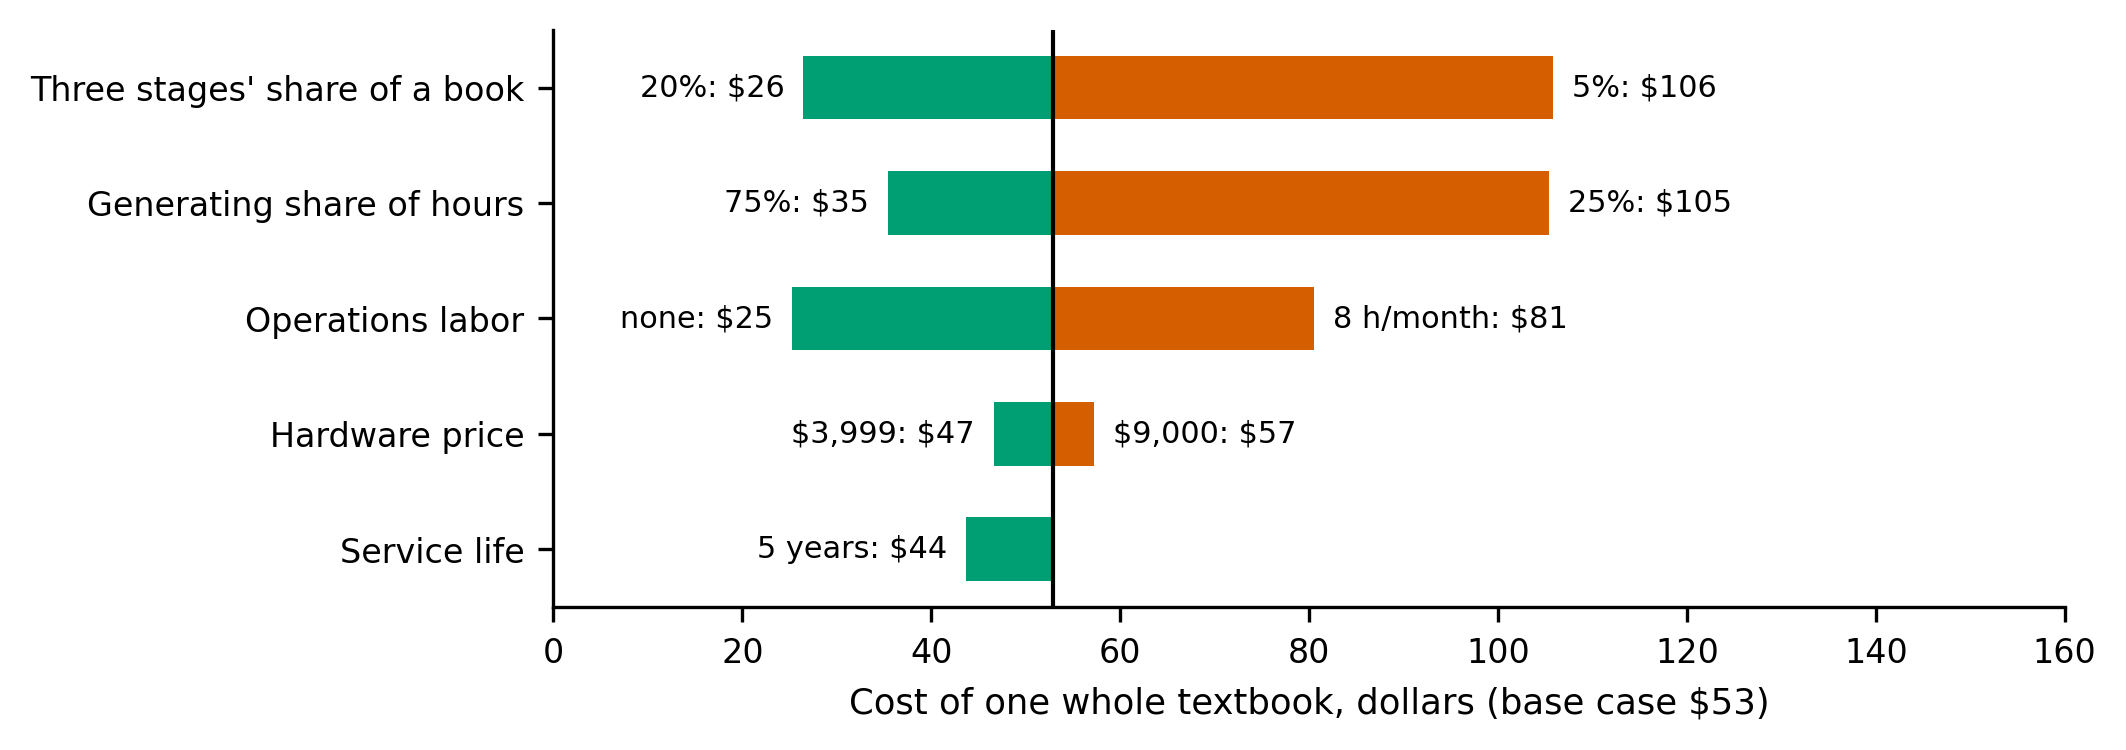
\includegraphics[width=0.95\textwidth]{figures/fig-cost-sensitivity.png}
\caption{One-at-a-time sensitivity of the cost of a whole textbook to each assumption, around the reference case. Bars to the left reduce the cost; bars to the right increase it.}
\label{fig:cost}
\end{figure}

\subsection{What the Price Leaves Out}

The model prices generation only. It excludes human review: ten hours of review by a subject expert at \$90 an hour adds \$900, seventeen times the cost of generating the book, and no output has yet been reviewed. It excludes the cloud supervision that started and watched these runs, which a service would replace with scripts at a cost not counted; it excludes selling, financing, and tax; and it excludes license terms, since several candidates state no license or attach conditions to commercial use. It also excludes a comparison with cloud generation of the same book, which would need token counts and timings that were not recorded for the published reference.

\section{Publishing Evidence from a Private Machine}
\label{sec:publishing}

An evaluation is meant to be shared, and the raw material behind it is not safe to share. The book and its source repository are public; the machines it evaluates are real, sit on a private network, and belong to someone else. Probe reports, command output, logs, and screenshots all carry addresses, host names, account names, and identifiers that make a machine easier to find, reach, or log in to. We treat publication as a security boundary and not as an afterthought, and the book teaches the practice as its last chapter.

\subsection{What Is Never Published}

The rule is that nothing in the repository or on the site may make the device under test easier to find, reach, or log in to, and it outranks realism and completeness: a sanitized example that looks less authentic is always the right trade. The excluded classes are: network addresses of the machines, the private network, and the author's own network; host names, mesh-network names, and the network's name; user names, passwords, and passphrases; SSH keys, network auth keys, API tokens, and model-hub tokens; log files and unedited command output; hardware identifiers such as serial numbers, GPU unique identifiers, and MAC addresses; and the access configuration of the real device, including its access-control policy, open ports, and firewall rules.

\subsection{Four Practices}

\paragraph{Placeholders and documentation ranges.}
Every example uses a placeholder (a host, a user, a network name) or an address from a range reserved for documentation. Sample output is edited by hand before it enters a chapter, including probe reports, GPU status output, and screenshots of terminals and admin consoles.

\paragraph{Raw output isolation.}
Run output stays outside the repository, and log files are ignored by version control. Hosts reach the scripts only through an environment variable, so no address is written into any file. The single automated path from run output to the book is a results publisher that copies only three kinds of file: a model's learning graph, its chapter text, and the course description. It leaves out any file that holds an address, a host name, or a home-directory path, and it counts what it removed so that the omission is visible. A narrow path with a blocklist beats a broad copy followed by cleaning because it fails closed: a file it does not recognize is left out.

\paragraph{Layered scanning.}
A pre-commit script inspects only the lines being added and matches addresses, mesh-network names, private-key headers, auth-key and token formats, home-directory paths, and serial-number and GPU-identifier lines, while allowing documentation ranges and the loopback address. A secret scanner can be run over the tree and over history \cite{gitleaks}. Both are layers and not a defense: a scanner finds credentials with a known shape and does not find an address in a paragraph or a host name in a caption, so a human reads the diff before every publish.

\paragraph{History persistence.}
A leak deleted in a later commit remains in every earlier commit, in every clone and fork made before the deletion, and in the deployed site and whatever indexes it. The order of operations follows: prevent rather than repair; if something sensitive has been committed, stop and tell the person responsible for the repository; treat any leaked credential as compromised; and regard history rewriting as a last resort that does not reach earlier copies.

\subsection{Applied to This Paper}

The numbers in this paper derive from logs but are counts and durations. The aggregation step copies no path, host name, session identifier, or text from the event streams, and its output was scanned for address-, host-, and path-like strings before it was committed. No figure contains an address, host name, or login, and the architecture diagram names the machines only as roles. The model-results pages that the book publishes contain only generated text.

\subsection{What Was Not Local}

One disclosure bears on the claim that generation never leaves the machine. The orchestrator, which started, watched, and scored runs, was a cloud model, and whatever it read to do so, including generated text, went to the cloud provider's API. The generation loop was local; its supervision was not. The harness was configured to send model requests only to the server on the same machine, with a placeholder credential and optional network features off, but that configuration was not confirmed with a packet capture. A deployment that needs the stronger property would replace the orchestrator with scripts and verify the network boundary.

\section{Discussion}
\label{sec:discussion}

\subsection{Findings}

\paragraph{F1: Completion, not prose quality, is the first-order obstacle.}
Four of ten models produced no learning graph, and four of the six that did did not finish stage~3. None of the stopped runs stopped because of how the prose read. The failures in Table~\ref{tab:failures} are failures to emit a well-formed tool call, to keep acting instead of announcing, to stay on task as the conversation fills the window, and to finish within a time limit. On this workload the ability that gates progress is protocol discipline over a long session, which is why the benchmark was framed around following a skill and calling tools and not around writing.

\paragraph{F2: A clean first stage did not predict a finished book.}
The cleanest learning graph came from the slowest model, which then wrote no chapter within the limit. The graph with the most duplicate labels, 40 of 200, came from the fastest model, which went on to write ten chapters. Stage~1 structural quality should not be used to choose a model for the whole pipeline, though with one run each this is an observation and not a rule.

\paragraph{F3: Sparse models were fastest, but speed did not buy completion.}
Both models that wrote every chapter activate about 3 billion parameters per token, and so does \Gtwentysix{} (3.8 billion), the fastest model, which wrote ten of fourteen. The largest sparse model, \Gptoss, ran at a usable speed and wrote six of ten. Architecture and speed are neither necessary nor sufficient for completion here; per-turn behavior, which the harness multiplies by hundreds of turns, matters more.

\paragraph{F4: Model-only tests did not predict harness behavior.}
\Gthirtyone{} passed every format rule in isolation and had the highest tool-call failure rate in the harness, 20\%. Model-only tests ran with reasoning off and the harness with each model's default, so the speeds measured in the first did not match the second. Two models wrote their first tool call as text in the harness, which may reflect a mismatch with the tool-call format the harness expects as much as an inability to call tools. The two layers of testing are not redundant; each finds failures the other cannot.

\paragraph{F5: Failures can be self-inflicted and can propagate across stages.}
Three of \Gtwentysix's chapter runs halted because the skill's own check found that a chapter depended on concepts placed in later chapters, and the chapter order that violated the dependency was the model's own stage~2 design. A cheap structural validation of the stage~2 output against the stage~1 graph would have found this in seconds, before ninety minutes of stage~3 per chapter. The benchmark chains stages by copying output forward, so a defect inherited from stage~2 is paid for once per chapter.

\paragraph{F6: The conformance score separates evenness from level, and shows its own limits.}
The headline separates two things that a mean would blur: \Gptoss{} is the most even book and the smallest, and \Nemo{} wrote the most and has the lowest floor. At the same time the score ties its top two books, cannot see that most of \Gptoss's words are specifications, and records that every book exceeds the target reading grade. It is a screen that points to chapters worth reading, not a verdict.

\paragraph{F7: On unified memory, context is a competitor to weights.}
\Mistral{} loaded and ran at 3 tokens per second and left no context of useful length. Two models drove a task to within about a thousand tokens of their configured window. One of the two units stopped responding twice during runs of the same model at large contexts. The cause was not established, and the second freeze at a smaller context makes memory exhaustion a weaker suspect than it first appeared, but the practical lesson holds: start a memory watchdog and a vitals log before any run, because a unified-memory machine can freeze instead of failing one process.

\subsection{Implications for Practitioners}

These follow from the observations above and are offered as practice, not as proof.

\begin{itemize}
\item \textbf{Gate on completion, then on quality.} Run a model-only test, then a three-minute harness smoke test, before any hour-long stage. A model that cannot call a tool in the harness will not finish a book.
\item \textbf{Budget time by turns, not tokens.} For the fast models the per-turn overhead exceeded generation time. Measure overhead per model; it ranged from 7 to 100 seconds here.
\item \textbf{Validate between stages.} Check each stage's output structurally before spending the next stage's budget on it.
\item \textbf{Treat a book-level score as a screen.} Read the chapters it flags, and do not choose a model on a headline that sits within the reweighting noise.
\item \textbf{Keep the evidence and the machine safe.} Isolate raw output, publish through a narrow path, and run the watchdog.
\end{itemize}

\subsection{Harness--Model Confound}

The harness is Claude Code, chosen because the published books were generated with it and the skills were written for it, so that the model is the only thing that changes. The cost is that its own instructions and tool definitions run to about 19,000 tokens and were written for Claude models. A local model that struggles may be struggling with the harness, not with the task. A second harness with a lighter prompt would separate a model failure from a harness mismatch, and is the most valuable single addition to this design.

\subsection{Threats to Validity}

\begin{itemize}
\item \textbf{One run per cell.} Run-to-run variance is unknown, and the ordering of models is not evidence. A second run could move a model from complete to incomplete or the reverse.
\item \textbf{No human judgment.} No person has judged whether any chapter is mathematically correct or pedagogically sound. The conformance score measures adherence to rules, and its thresholds were read off the same six books it now scores, so the score is not independent of the corpus.
\item \textbf{No cloud baseline.} The published reference book was made with earlier skills and no timings were kept, so the paper cannot say how a local model compares with a cloud model under identical conditions.
\item \textbf{Uncontrolled variables.} Context length, reasoning mode, and server behavior differed across models (Table~\ref{tab:controls}); one server's re-reading may have penalized one model for reasons that are not the model's.
\item \textbf{Time limits are choices.} A model that wrote nothing in two 90-minute runs might finish in 180 minutes; ``wrote no chapter'' is relative to the limit.
\item \textbf{A lenient definition of written.} A chapter counts as written with at least 1,000 words and no placeholder; the score then measures how well it conforms.
\item \textbf{Assistant-made decisions.} An AI assistant chose the candidate list, the model server, and the scoring methods under the author's direction. The design-choices page attributes each decision, but the assistant's blind spots are in the benchmark too.
\item \textbf{One machine, one course, one skill version.} Nothing here generalizes to another course, another skill version, or another hardware class without a rerun. Publisher claims about models were not checked.
\end{itemize}

\subsection{Responsible Use}

The opportunities and risks of large language models in education are well surveyed \cite{kasneci2023chatgpt}, and the central caution applies here with full force: generated educational content must be reviewed by a subject expert before it reaches learners. Local generation changes where data goes, not whether the text is correct. The book labels its generated content as unreviewed; its MicroSims are implemented but not approved; and its model-results pages are shown as each model wrote them. The conformance score should not be used to grade a person's work, and it was not designed for that.

\section{Conclusion}
\label{sec:conclusion}

We asked whether open-weight models small enough to run on one 128~GB workstation can generate an intelligent textbook without sending a token to the cloud. In a first, single-run round of ten models on one DGX Spark-class unit, six produced a learning graph, all six ran all three stages, and two wrote every chapter they had designed, in about two to three machine hours. The others stopped for reasons that were mostly about protocol and persistence over a long session and not about prose: tool calls written as text, work announced and not done, a lost task, a time limit, or a context that did not fit. The cleanest learning graph came from the slowest model, and a clean first stage did not predict a finished book.

We offered five artifacts alongside the measurements: a reproducible benchmark definition; a deterministic chapter-conformance score that favors even quality and states its own limits; a cost model whose inputs were checked against measured time and found to agree only partly by cancellation; a 23-chapter open textbook that teaches the method; and a publication discipline for evidence from private hardware.

The evidence is thin by design and should be read that way. Each model ran each stage once, no person has judged whether the chapters are correct, the conformance score has not been compared with human ratings, and there is no cloud baseline. The paper therefore supports a statement about feasibility, that a local model on one machine can complete the pipeline, and withholds any statement about equivalence.

\subsection{Future Work}

The next steps follow directly from the limits above, in the order that would most reduce uncertainty.

\begin{enumerate}
\item \textbf{Repeated runs.} At least three, preferably five, runs of each completed configuration, to report a range and not a point, and a control run to check the apparatus.
\item \textbf{Blind human review.} Have subject experts rate a sample of chapters, about ten to twenty, without knowing the producing model, to calibrate or replace the score's weights and to judge correctness.
\item \textbf{A cloud baseline.} Generate the same book with a cloud model under the same prompts and skills, with token counts and timings recorded, and score it with the same program.
\item \textbf{A second harness.} Run the same models under a harness with a lighter prompt to separate model failure from harness mismatch.
\item \textbf{Throughput and precision.} Test a batching server such as vLLM on the best candidate, and an 8-bit quantization of the models that completed.
\item \textbf{The remaining stages and other courses.} Extend to MicroSims, the glossary, FAQ, quizzes, and references, and to a second course, to test whether the thresholds and the stage ordering carry over.
\item \textbf{Energy at the wall.} Replace the assumed power draw with a measured one.
\end{enumerate}

\noindent The book, its source, the aggregated run data, and the scripts that regenerate every number and figure in this paper are public at \url{https://github.com/dmccreary/dgx-eval}; the raw run output is deliberately not.


% Acknowledgments
\section*{Acknowledgments}
The author thanks the administrator of the DGX units for hosting the evaluation and for investigating the machine that stopped responding, and the open-source communities behind Ollama, llama.cpp, MkDocs Material, and p5.js on which the work depends.

\paragraph{Use of AI assistance.}
An AI assistant (Claude, Anthropic) built the test harness and scripts, ran the benchmark, wrote most of the book, and drafted this manuscript from the book's pages and the run records, under the author's direction. The decisions it made and the ones the author made are recorded and attributed in the book's design-choices page. Every number, table, and figure in this paper was regenerated by program from the repository. The author is responsible for the content.


% References
\bibliographystyle{ieeetr}
\bibliography{sections/references}

\end{document}
